%
% CHAPTER: Machine Learning
%

\chapterimage{Capek_play.pdf}

\chapter{Machine Learning}
\label{chap:Machine-Learning}

\begin{quote}
\begin{flushright}
\emph{There are no difficult problems,\\
only lack of imagination.}\\
Antonio García \\
\end{flushright}
\end{quote}
\bigskip

We have seen that the most difficult problems to which we can apply the results of the theory of nescience arise when set of entities $\mathcal{E}$ under study is composed by abstract elements. The difficulty with abstract entities is that it does not exits a way to encode them as strings of symbols so we can effectively reconstruct them. In practice, a possible approach to deal with this problem is to run an experiment and collect the results, as we do in case of physics. An alternative approach would be to take a collection of measurements, like for example, by means of observing the behavior of users in an online social network.

This chapter is devoted to how to apply the concept of minimum nescience to the area of machine learning. We assume that the entities under study are encoded as a dataset $\mathbb{X}$ composed by $n$ training vectors of $p$ predictors and a response variable $\bold{y}$ (see Section \ref{sec:machine_learning}).

We will start by providing practical approximations for the concepts of miscoding, inaccuracy and surfeit when the entities are encoded as datasets, and then we will show how to combine them in the single quantity of nescience. These approximations will allow us to introduce the \emph{minimum nescience principle}, a technique designed to automate the process of finding optimal models in machine learning (auto-machine learning). 

Besides introducing these approximations, we will show how to apply them to solve practical problems. The examples will be based on the \texttt{nescience}\footnote{\texttt{https://github.com/rleiva/nescience}} library, an open source python library that provides an implementation of the ideas included in this chapter.

%
% Section: Nescience Library
%

\section{Nescience Python Library}

The \texttt{nescience} library is an open source Python library that provides an implementation of the ideas included in this book applied to the area of machine learning. The library follows the API and conventions of the highly popular \texttt{scikit-learn} machine learning tool suite, and so, it can be combined with the methods provided by this package.

The \texttt{nescience} library can be installed with the \texttt{pip} utility:

\begin{sourcecode}
{\scriptsize \begin{verbatim}
pip install nescience
\end{verbatim}}
\end{sourcecode}

In the web page that accompanies this book, the reader can find a collection of notebooks for the \texttt{jupyter-lab} environment describing how the library works. For each subsection of this chapter, there is a notebook that implements all the examples included, so that the reader can repeat and play with them. Additional information about the \texttt{nescience} library, and a reference of the API provided, can be also found in the web page of the book.

%
% Section: A Note About Compression
%
\section{A Note About Compression}
\label{sec:note_about_compression}

As it is customary, the Kolmogorov complexity $K(s)$ of a string $s$ will be approximated by the length of the compressed version of that string using a standard compressor, that is, we will use the normalized compression distance:
\[
E_Z(\mathbf{x}_j, \mathbf{y}) = \frac{\max\{ \hat{K}_Z(\mathbf{x}_j \mid \mathbf{y}), \hat{K}_Z(\mathbf{y} \mid \mathbf{x}_j) \}}{\max \{ \hat{K}_Z(\mathbf{x}_j), \hat{K}_Z(\mathbf{y}) \} }
\]
where $\hat{K}_Z(s)$ denotes the length of the compressed version of the string $s$ using the compressor $Z$. In the particular case of having a vector $\mathbf{x} = \{ x_1, \ldots, x_n \}$ of measurements, the string $s$ to be compressed will be the concatenation of the encoded values $s = \langle x_1, \ldots, x_n \rangle$. We prefer the following equivalent definition of normalized compression dinstance, since in practice it is easier to compute the joint distribution of two vectors than the conditional distribution:
\[
E_Z(\mathbf{x}_j, \mathbf{y}) = \frac{ \hat{K}_Z(\mathbf{x}_j, \mathbf{y}) - \min\{ \hat{K}_Z(\mathbf{x}_j), \hat{K}_Z(\mathbf{y}) \} } { \max\{ \hat{K}_Z(\mathbf{x}_j), \hat{K}_Z(\mathbf{y}) \} }
\]
As compression technique we will use a code $C$ with minimal length, given the relative frequencies of the different observed values (see Section \ref{sec:Optimal-Codes}). If $\mathbf{x}$ is a qualitative vector (either a feature or the target variable) taking values from a set labels $\mathcal{G} = \{g_1, \ldots, g_\ell\}$, that is $\mathbf{x} \in \mathcal{G}^n$, the quantity $\hat{K}_C(\mathbf{x})$ can be computed as:
\[
\hat{K}_C(\mathbf{x}) = - \sum_{i=1}^l \log_2{ \frac{ \sum_{j=1}^n I(x_j = g_i)} {n} } 
\]
If the case of $\mathbf{x}$ being based on a continuous random variable, we cannot calculate the probability of $x_j$ since, in general, the underline probability distribution of $\mathbf{x}$ is unknown. Moreover, we have that $P(x_j)=0$ for all $j$. In order to approximate the value $K(\mathbf{x})$ using a minimal length code $C$, we have to discretize first the vector $\mathbf{x}$ into a collection of intervals.

A discretization algorithm is a mapping between a (possibly huge) number of numeric values and a reduced set of discrete values, and so, it is a process in which some information is potentially lost. The choice of discretization algorithm is something that could have a high impact in the practical computation of the nescience. We are interested in a discretization algorithm that produces a large number of intervals (low bias), with a large number of number of observations per interval (low variance). Common techniques include \emph{equal width discretization}, \emph{equal frequency discretization} and \emph{fixed frequency discretization}. However, these techniques require the optimization of an hyperparameter, and so, they are not suitable for our purposes.

In the \texttt{nescience} library we use a proportional discretization approach (see Section \ref{sec:discretization_algorithms}), where the number of intervals $m$ and the number of observations per interval $s$ are equally proportional to the number of observations $n$. In particular, in the nescience library we set $s = m = \sqrt{n}$.

Using this discretization procedure, we can approximate the Kolmogorov complexity of a vector $\mathbf{x}$ by:
\[
\hat{K}_C(\mathbf{x}) = - \sum_{i=1}^m \log_2{ \frac{ \sum_{j=1}^n I(x_j \in D_i)} {n} } 
\]
where $D_i$ is the interval defined by the end points $(i-1, i)$.

The quantity $\hat{K}_C$ can be generalized to the an arbitrary number of $m$ vectors $\hat{K}_C(\mathbf{x_1}, \ldots, \mathbf{x_m})$ composed by $n$ samples each, by considering the joint encoded vector
\[
\langle \mathbf{x_1}, \mathbf{x_2}, \ldots, \mathbf{x_m} \rangle = \{ \langle x_{11}, x_{12}, \ldots, x_{1m} \rangle, \ldots, \langle x_{n1}, x_{n2}, \ldots, x_{nm} \rangle \}
\]

\begin{proposition}
The normalized compression distance of two vectors $x$ and $y$ computed using a compressor based on optimal codes is equivalent to the normalized mutual information of these two vectors, that is:
\[
NCD_C\left(\mathbf{x},\mathbf{y}\right)=1-\frac{I\left(\mathbf{x};\mathbf{y}\right)}{\max\left\{ H\left(\mathbf{x}\right),H\left(\mathbf{y}\right)\right\} }
\]
\end{proposition}
\begin{proof}
We have to prove that
\begin{align*}
NCD\left(\mathbf{x},\mathbf{y}\right) & = \frac{C\left(\mathbf{x},\mathbf{y}\right)-\min\left\{ C\left(\mathbf{x}\right),C\left(\mathbf{y}\right)\right\} }{\max\left\{ C\left(\mathbf{x}\right),C\left(\mathbf{y}\right)\right\} } =\frac{nH\left(\mathbf{x},\mathbf{y}\right)-\min\left\{ nH\left(\mathbf{x}\right),nH\left(\mathbf{y}\right)\right\} }{\max\left\{ nH\left(\mathbf{x}\right),nH\left(\mathbf{y}\right)\right\} } \\
& =\frac{H\left(\mathbf{x},\mathbf{y}\right)-\min\left\{ H\left(\mathbf{x}\right),H\left(\mathbf{y}\right)\right\} }{\max\left\{ H\left(\mathbf{x}\right),H\left(\mathbf{y}\right)\right\} }
\end{align*}
We have to consider two cases. In case 1 we assume that $H\left(\mathbf{x}\right)>H\left(\mathbf{y}\right)$, and so
\begin{align*}
NCD\left(\mathbf{x},\mathbf{y}\right) & = \frac{H\left(\mathbf{x},\mathbf{y}\right)-H\left(\mathbf{y}\right)}{H\left(\mathbf{x}\right)} = \frac{H\left(\mathbf{y}\right)+H\left(\mathbf{x}\mid\mathbf{y}\right)-H\left(\mathbf{y}\right)}{H\left(\mathbf{x}\right)} = \frac{H\left(\mathbf{x}\mid\mathbf{y}\right)}{H\left(\mathbf{x}\right)} \\
& = \frac{H\left(\mathbf{x}\right)-\left(H\left(\mathbf{x}\right)-H\left(\mathbf{x}\mid\mathbf{y}\right)\right)}{H\left(\mathbf{x}\right)} = 1-\frac{I\left(\mathbf{x};\mathbf{y}\right)}{H\left(\text{\ensuremath{\mathbf{x}}}\right)}
\end{align*}
and in case of $H\left(\mathbf{y}\right)>H\left(\mathbf{x}\right)$ we have that
\begin{align*}
NCD\left(\mathbf{x},\mathbf{y}\right) & = \frac{H\left(\mathbf{x},\mathbf{y}\right)-H\left(\mathbf{x}\right)}{H\left(\mathbf{y}\right)} =\frac{H\left(\mathbf{x}\right)+H\left(\mathbf{y}\mid\mathbf{x}\right)-H\left(\mathbf{x}\right)}{H\left(\mathbf{y}\right)} = \frac{H\left(\mathbf{y}\mid\mathbf{x}\right)}{H\left(\mathbf{y}\right)}=\frac{H\left(\mathbf{y}\right)-\left(H\left(\mathbf{y}\right)-H\left(\mathbf{x}\mid\mathbf{y}\right)\right)}{H\left(\mathbf{y}\right)} \\
& = \frac{H\left(\mathbf{y}\right)-\left(H\left(\mathbf{y}\right)-H\left(\mathbf{x}\mid\mathbf{y}\right)\right)}{H\left(\mathbf{y}\right)} = 1-\frac{I\left(\mathbf{x};\mathbf{y}\right)}{H\left(\text{\ensuremath{\mathbf{y}}}\right)}
\end{align*}
and so
\[
NCD_c\left(\mathbf{x},\mathbf{y}\right)=1-\frac{I\left(\mathbf{x};\mathbf{y}\right)}{\max\left\{ H\left(\mathbf{x}\right),H\left(\mathbf{y}\right)\right\} }
\]
\end{proof}

The quantity $1 - \frac{I\left(\mathbf{x};\mathbf{y}\right)}{\max\left\{ H\left(\mathbf{x}\right),H\left(\mathbf{y}\right)\right\} }$ has been already proposed in~\cite{ferri2009experimental} as a candidate definition of the concept of Normalized Mutual Information. However, to the best of our knowledge, it has not been used in practice.

\begin{example}
    
\end{example}

\begin{remark}
    
In order to properly approximate the complexity of a continuos feature, we have to use a discretization algorthm that does not change the distribution of the observed values. For example, the kmeans algorithm, given that the optimization criteria es to minimize 


In the \texttt{nescience} we use a uniform discretization, in which all the intervals have the same length. However, this apprach is not optimal, especially when we are in a two dimensional space, in which we have to discretize the joint distribution of two attributes x and y. 

For example, in the next figure, we can see a cloud of points, and how a uniform distriubtion has many intervals withour points.

\begin{figure}[ht]
    \centering
    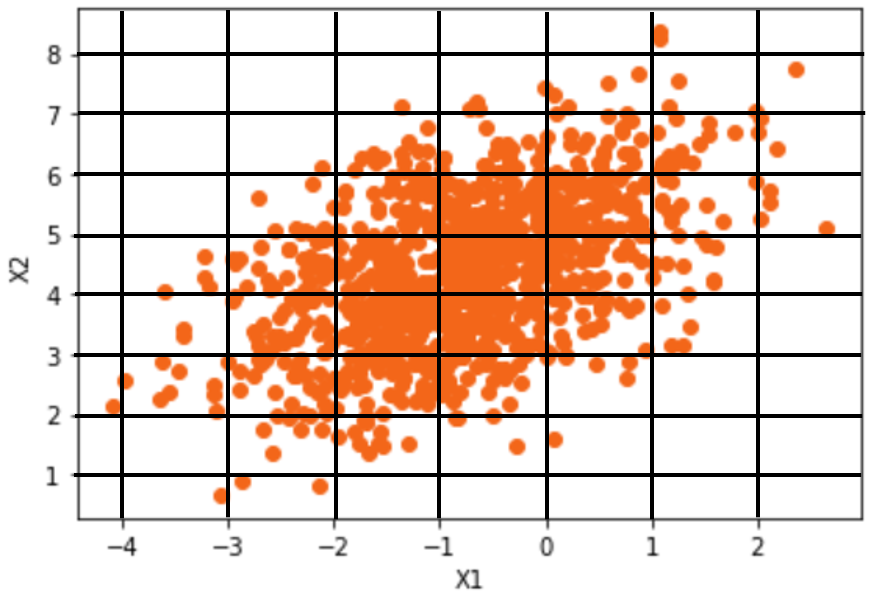
\includegraphics[width=0.6\textwidth]{discretization_uniform.png}
    \caption{Uniform discretization.}
    \label{figure:discretization_uniform}
\end{figure}

A better approach would be to compute the convex hull arund the actual cloud of points, and then divide the space into sqrt intervals of the same length, by for example, computing the n centroid using a kmeans algorithm and then useing voronoi pologons. Howerver, up to the best of our knowledge, a discretization algorithm based on a constrained version of the kmeans in which the distribution of the points is not changes, has not been developed.

\begin{figure}[ht]
    \centering
    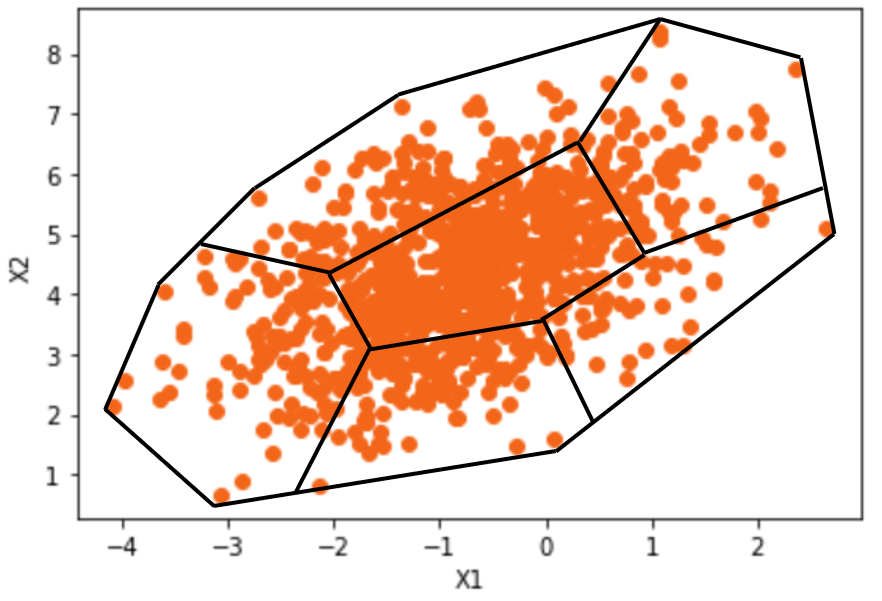
\includegraphics[width=0.6\textwidth]{discretization_kmeans.png}
    \caption{Convex hull and kmeans discretization.}
    \label{figure:discretization_kmeans}
\end{figure}


\end{remark}

%
% Section: Miscoding
%

\section{Miscoding}
\label{sec:machine_learning_miscoding}

In Section \ref{def:miscoding} we introduced the concept of miscoding as a quantitative measure of how well a string based encoding $r \in \mathcal{R}$ represents a research entity from $\mathcal{E}$. The miscoding of a representation $r$ was defined as:
\[
\mu(r) = \overset{o}{ \underset{s \in \mathcal{R}_\mathcal{E}} \min} \frac{ \max\{ K(s \mid r), K(r \mid s) \} } { \max\{ K(s), K(r) \} }
\]
and we saw that this quantity cannot be computed in practice for the general case. First of all because it requires a computation from an abstract oracle machine, second because it is based on the uncomputable Kolmogorov complexity, and third because it does not take into account the entity $e$ in which we are interested. 

In this section we are going to see how this concept can be adapted in practice to compute the error made by using a dataset $\mathbf{X}$ as a representation of a response variable $\mathbf{y}$ (see Section \ref{sec:machine_learning}). Our goal is double, in one hand we are interested in measuring the quality of the dataset $\mathbf{X}$ as a predictor of the variable $\mathbf{y}$, and in the other we want to identify those features $\mathbf{x}_j$ of $\mathbf{X}$ that have the higher predictive power for $\mathbf{y}$. This is the problem addressed by discriminative models (see Section \ref{sec:generative_discriminative}) in which we want to estimate the conditional distribution $P( \mathbf{y} \mid \mathbf{X} )$.

Given a training dataset $\mathbf{X}$, we can approximate the miscoding of a feature $\mathbf{x}_j$ for the target variable $\mathbf{y}$ by computing the normalized information distance between $\mathbf{x}_j$ and $\mathbf{y}$ (see Section \ref{sec:information_distance}):
\[
E(\mathbf{x}_j, \mathbf{y}) = \frac{\max\{ K(\mathbf{x}_j \mid \mathbf{y}), K(\mathbf{y} \mid \mathbf{x}_j) \}}{\max \{ K(\mathbf{x}_j), K(\mathbf{y}) \} }
\]
The Kolmogorov complexity $K(\mathbf{v})$ of a vector $\mathbf{v}$ will be approximated by the length of the compressed version of that vector $\hat{K}_C(\mathbf{v})$ using as compressor a minimal length code $C$ (see Section \ref{sec:note_about_compression}).

\begin{definition}
Let $\mathbf{y}$ be a response variable, $\mathbf{X}$ a dataset composed by $p$ features, and $\mathbf{x}_j$ the $j-th$ feature. We define the regular feature miscoding of $\mathbf{x}_j$ as a representation of $\mathbf{y}$, denoted by $\hat\mu(\mathbf{x}_j, \mathbf{y})$, as:
\[
\hat\mu(\mathbf{x}_j, \mathbf{y}) = \frac{ \hat{K}_C(\mathbf{x}_j, \mathbf{y}) - \min\{ \hat{K}_C(\mathbf{x}_j), \hat{K}_C(\mathbf{y}) \} } { \max\{ \hat{K}_C(\mathbf{x}_j), \hat{K}_C(\mathbf{y}) \} }
\]\end{definition}

Intuitively, the quantity $\hat\mu(\mathbf{x}_j, \mathbf{y})$ is a measure of the effort, as the length of a computer program and in relative terms, required to fully encode $\mathbf{y}$ assuming a knowledge of $\mathbf{x}_j$, and the other way around. The lower this value, the better would be the quality of $\mathbf{x}_j$ as a predictor for $\mathbf{y}$.

\begin{example}

Let's $\mathbf{y}$ be a target variable composed by $1.000$ random samples that follows a normal distribution $N(3,1)$ with mean $\mu = 3$ and standard deviation $\sigma = 1$, $\mathbf{x}_1$ be a predictor feature that is equal to $\mathbf{y}$ with some random noise, that is $\mathbf{x}_1 = \mathbf{y} + N(3, 1) / 10$, and $\mathbf{x}_2$ be a second predictor based on random samples from a exponential distribution with a rate of $\lambda = 1$.

\begin{sourcecode}
{\scriptsize \begin{verbatim}
from scipy.stats import norm, expon

y  = norm.rvs(loc=3, scale=1, size=10000)
x1 = y + norm.rvs(loc=3, scale=1, size=10000) / 10
x2 = expon.rvs(size=10000)
\end{verbatim}}
\end{sourcecode}

We can use the Nescience library to compute the miscoding of the features $\mathbf{x}_1$ and $\mathbf{x}_2$ when they encode the target variable $\mathbf{y}$.

\begin{sourcecode}
{\scriptsize \begin{verbatim}
from fastautoml.miscoding import Miscoding
import numpy as np

X = np.column_stack((x1, x2))

miscoding = Miscoding()
miscoding.fit(X, y)
miscoding.miscoding_features(mode="regular")
\end{verbatim}}
\end{sourcecode}

The output of the library would be something similar to the following\footnote{Since we are generating a list of $1.000$ random samples, the reader could get a slightly different result when running this example.}:

\begin{sourcecode}
{\scriptsize \begin{verbatim}
array([0.27445364, 0.9934222])
\end{verbatim}}
\end{sourcecode}

As it was expected the miscoding of $\hat\mu(\mathbf{x}_1, \mathbf{y})$ is much smaller than the miscoding of $\hat\mu(\mathbf{x}_2, \mathbf{y})$. In this case, we should prefer $\mathbf{x}_1$ over $\mathbf{x}_2$ as a predictor of $\mathbf{y}$.

\end{example}

Sometimes we will use the normalized version of the complements of the individual miscodings, that is $\frac{ 1 - \hat\mu(\mathbf{x}_i, \mathbf{y}) } { \sum_{i=j}^p 1 - \hat\mu(\mathbf{x}_j, \mathbf{y}) }$, instead of the regular ones $\hat\mu(\mathbf{x}_i, \mathbf{y})$, because they are easier to compare with other feature selection techniques, and because they have a visually appealing interpretation. We call this version of miscoding the \emph{adjusted} feature miscoding.

\begin{example}
\label{example:gaussian_blob_miscoding}
In this example we are going to generate a synthetic dataset where the target variable $\mathbf{y}$ is a collection of normally-distributed clusters of points, and the training set $\mathbb{X}$ is composed by both, relevant and irrelevant predictors. In particular we will generate $1.000$ samples composed by $20$ features that describe $10$ clusters; only $4$ of the features are relevant for prediction, and the other remaining $6$ are just random values.

In Figure \ref{figure:gaussian_blob_cluster} we can see a two-dimensional projection of this dataset, along the hyperplane composed by features 8 and 10.

\begin{figure}[h]
\centering
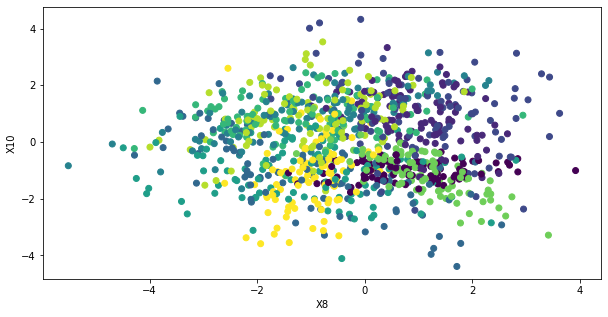
\includegraphics[width=0.6\textwidth]{gaussian_blob_cluster.png}
\caption{Gaussian Blob Cluster.}
\label{figure:gaussian_blob_cluster}
\end{figure}

\begin{sourcecode}
{\scriptsize \begin{verbatim}
from fastautoml.miscoding import Miscoding
from sklearn.datasets.samples_generator import make_classification

X, y = make_classification(n_samples=1000, n_features=20, n_informative=4,
       n_redundant=0, n_classes=10, n_clusters_per_class=1, flip_y=0)

miscoding = Miscoding()
miscoding.fit(X, y)
msd = miscoding.miscoding_features(mode='adjusted')
\end{verbatim}}
\end{sourcecode}

We will use the adjusted version of the miscoding for an easier comparison with other feature selection techniques. If we plot the results (see Figure \ref{figure:miscoding_make_classification}) we will see that the library has successfully identified the four relevant predictors ($\mathbf{x}_3$, $\mathbf{x}_8$, $\mathbf{x}_{10}$ and $\mathbf{x}_{16}$). Since we are using the adjusted version of miscodings, the higher the value the better, and mind that actual values have to be interpreted in relative terms. 

\begin{figure}[h]
\centering
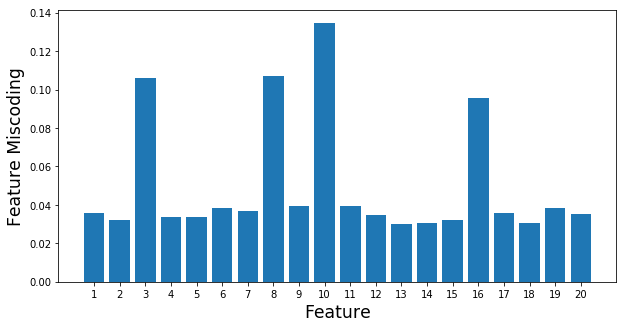
\includegraphics[width=0.6\textwidth]{feature_miscoding.png}
\caption{Miscoding of a Synthetic Dataset.}
\label{figure:miscoding_make_classification}
\end{figure}

We can compare miscoding with correlation, a common technique used in machine learning to identify the most relevant features of a dataset. In Figure \ref{figure:correlation_make_classification} is shown correlation between the individual features that compose $\mathbf{X}$ and the target variable $\mathbf{y}$. As we can observe, correlation fails to properly identify one of the relevant features ($\mathbf{x}_3$).

\begin{figure}[h]
\centering
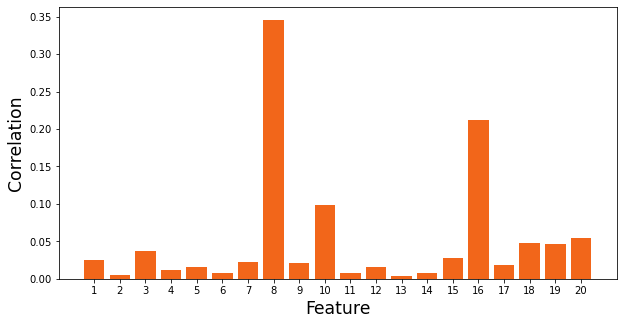
\includegraphics[width=0.6\textwidth]{feature_correlation.png}
\caption{Correlation of a Synthetic Dataset.}
\label{figure:correlation_make_classification}
\end{figure}

\end{example}

Feature miscoding allow us to identify the most relevant features of a training dataset $\mathbf{X}$, but it cannot be used to compute the miscoding of the dataset itself. If we start with a miscoding of $1$ (full unknown), and subtract the miscodings of the individual features, we will end up with a negative miscoding, something that it is not allowed by our theory. If we use the adjusted version, the dataset miscoding will be $0$ for all datasets, which is against our intuition that not all possible datasets $\mathbf{X}$ represent equally well a target variable $\mathbf{y}$. According to the theory of nescience, we expect that non-relevant features add, instead of subtract, to the global miscoding of the dataset.

In order to address this problem, we have to introduce the concept of partial miscoding of a feature, as the difference between the adjusted and normalized miscodings.

\begin{definition}
Let $\mathbf{y}$ be a target variable, $\mathbf{X}$ a dataset composed by $p$ features, and $\mathbf{x}_j$ the $j-th$ feature. We define the partial miscoding of $\mathbf{x}_j$ as a representation of $\mathbf{y}$, denoted by $\tilde\mu(\mathbf{x}_j, \mathbf{y})$, as:
\[
\tilde\mu(\mathbf{x}_i, \mathbf{y}) = \frac{ 1 - \hat\mu(\mathbf{x}_i, \mathbf{y}) } { \sum_{j=1}^p 1 - \hat\mu(\mathbf{x}_j, \mathbf{y}) } - \frac{\hat\mu(\mathbf{x}_i, \mathbf{y}) } { \sum_{j=1}^p \hat\mu(\mathbf{x}_j, \mathbf{y}) }
\]
\end{definition}

A positive partial miscoding means that the feature contributes to describe the target variable, meanwhile a negative value means that the feature is not relevant.

\begin{example}
\label{example:partial_feature_miscoding}
We will use again the synthetic dataset of Example \ref{example:gaussian_blob_miscoding}, but we will increase the number of relevant features from $4$ to $14$. Then, we will compute the list of partial miscodings.

\begin{sourcecode}
{\scriptsize \begin{verbatim}
from fastautoml.miscoding import Miscoding
from sklearn.datasets.samples_generator import make_classification

X, y = make_classification(n_samples=1000, n_features=20, n_informative=14,
       n_redundant=0, n_classes=10, n_clusters_per_class=1, flip_y=0)

miscoding = Miscoding()
miscoding.fit(X, y)
msd = miscoding.miscoding_features(mode="partial")
\end{verbatim}}
\end{sourcecode}

As we can see in Figure \ref{figure:partial_feature_miscoding}, not only the library has been able to correctly identify the relevant features, but also, non relevant features have now a negative contribution to the global miscoding.

\begin{figure}[h]
\centering
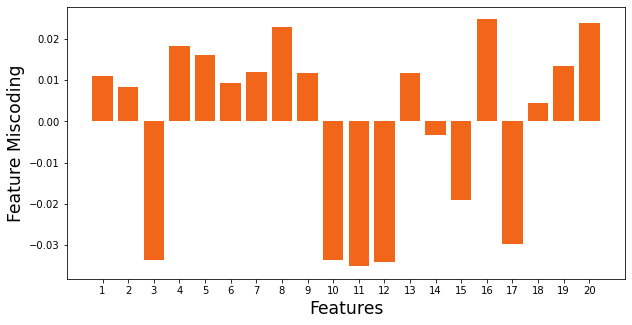
\includegraphics[width=0.6\textwidth]{partial_miscoding.png}
\caption{Partial Feature Miscoding.}
\label{figure:partial_feature_miscoding}
\end{figure}

\end{example}

Given the definition of partial feature miscoding we can provide a definition of the concept of miscoding of a target variable given a subset of predictors that it is closer to the original concept of miscoding defined by the theory of nescience.

\begin{definition}
Let $\mathbf{y}$ be a target variable, $\mathbf{X} = \{ \mathbf{x}_1, \ldots, \mathbf{x}_p \}$ a dataset composed by $p$ features, and $\mathbf{Z} = \{ \mathbf{z}_1, \ldots, \mathbf{z}_k \}$ a subset of features, that is, $\{ \mathbf{z}_1, \ldots, \mathbf{z}_k \} \subseteq \{ \mathbf{x}_1, \ldots, \mathbf{x}_p \}$. We define the miscoding of $\mathbf{Z}$ as a representation of $\mathbf{y}$, denoted by $\hat\mu(\mathbf{Z}, \mathbf{y})$, as:
\[
\hat\mu(\mathbf{Z}, \mathbf{y}) = \sum_{i=1}^k \tilde\mu (\mathbf{z}_i, \mathbf{y})
\]
\end{definition}

\begin{example}
\label{example:accumulated_partial_feature_miscoding}
Based on the dataset and the partial features miscoding computed in Example \ref{example:partial_feature_miscoding}, in Figure \ref{figure:accumulated_partial_feature_miscoding} we can see the evolution of the miscoding of the training subset $\mathbf{Z}$ as we add more features to the study.

\begin{figure}[h]
\centering
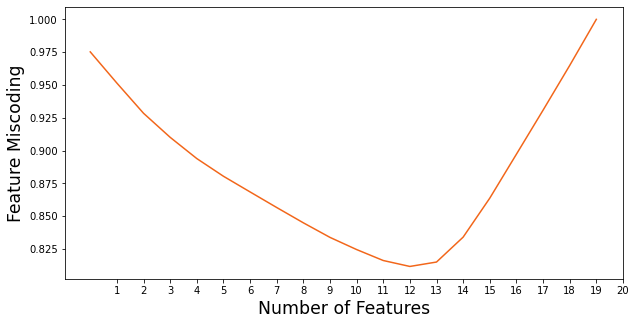
\includegraphics[width=0.6\textwidth]{accumulated_partial_miscoding.png}
\caption{Accumulated Partial Feature Miscoding.}
\label{figure:accumulated_partial_feature_miscoding}
\end{figure}

\end{example}

In the following example we are going to compare the performance of a machine learning classifier when using a full dataset and a reduced version of the same dataset using only those features identified as relevant, i.e., with positive partial miscoding.

\begin{example}
Let's train a neural network with the standard MNIST dataset in order to classify hand written digits. The evaluation criteria will be the score of the classifier, that is, the percentage of digits correctly classified, applied over a test dataset different from the dataset used for training. The neural network will be trained and evaluated using all the features that compose the dataset, and with a reduced version of the dataset composed by only those features with a positive partial miscoding.

\begin{sourcecode}
{\scriptsize \begin{verbatim}
import numpy  as np
from sklearn.model_selection import train_test_split
from sklearn.neural_network import MLPClassifier
from sklearn.datasets import load_digits
from fastautoml.fastautoml import Miscoding

data = load_digits()
X_raw = data.data
y_raw = data.target

miscoding = Miscoding()
miscoding.fit(X_raw, y_raw)
mscd = miscoding.miscoding_features(miscoding='partial')
X_red = X_raw[:,np.where(mscd > 0)[0]]
y_red = y_raw

X_raw_train, X_raw_test, y_raw_train, y_raw_test = train_test_split(X_raw,
             y_raw, test_size=.3)
X_red_train, X_red_test, y_red_train, y_red_test = train_test_split(X_red,
             y_red, test_size=.3)

clf = MLPClassifier(alpha=1, max_iter=1000)

clf.fit(X_raw_train, y_raw_train)
score_raw = clf.score(X_raw_test, y_raw_test)
        
clf.fit(X_red_train, y_red_train)
score_red = clf.score(X_red_test, y_red_test)
        
reduction = 1 - X_red_train.shape[1] / X_raw_train.shape[1]

print("Score raw:", score_raw, " Score Miscoding:", score_red,
      " Reduction:", reduction)

Score raw: 0.9833333333333333  Score Miscoding: 0.9814814814814815  Data Reduction: 0.46875
\end{verbatim}}
\end{sourcecode}

If we run the above source code, we will see that the score of the neural network classifier is about the same for the two datasets, 98\% of the digits are correctly classified using the test data. However, the reduced dataset used for training based on the optimal miscoding is 43\% smaller than the original dataset. This size reduction could have a big impact in the training time of the neural network. Smaller datasets are also relevant when working with ensembles of models, like random forests, where hundreds or thousands of models have to be trained.

\end{example}

Intuitively, as Example \ref{example:accumulated_partial_feature_miscoding} shows, we should prefer the subset $\mathbf{Z}$ of $\mathbf{X}$ composed by all those features whose partial miscoding are greater than zero. However, as we will see in the following sections of this chapter, this might not be the case. Feature selection is only one of the criteria used in the process of finding an optimal model for an entity represented by a dataset. It might happen that other elements, like inaccuracy or surfeit, suggest to use a different subset of predictors. The global optimization criteria we should use is the concept of nescience. A sensible approach to use partial miscoding would be to incrementally add to our model those features with higher miscoding, until all features with a positive value have been added, or an optimality criterion has been reached.

In case of having a generative model (see Section \ref{sec:generative_discriminative}), that is, a machine learning algorithm designed to find the joint probability $P(\mathbf{X}, \mathbf{y})$, we could use miscoding to compute how the different features relate to each other, that is, the quantity $\hat\mu(\mathbf{x}_i, \mathbf{x}_j)$ for each pair of values $i, j \leq p$. The result would be a miscoding matrix (see Example \ref{example:miscoding_boston}).

\begin{example}
\label{example:miscoding_boston}
The Boston dataset included in \texttt{scikit-learn} library contains a collection of variables that (potentially) could explain the price of houses in the area of Boston. In this example, instead of computing which are the factors that contribute the most to the price of houses, we are going to study the inter-dependence between these factors, using a miscoding matrix.

\begin{sourcecode}
{\scriptsize \begin{verbatim}
from fastautoml.fastautoml import Miscoding
from sklearn.datasets import load_boston

data = load_boston()

miscoding = Miscoding(X_type="numeric", y_type="numeric")
miscoding.fit(data.data, data.target)
mscd_matrix = miscoding.features_matrix(mode='regular')
\end{verbatim}}
\end{sourcecode}

In Figure \ref{figure:miscoding_matrix} we can see a graphical representation using a heatmap of the miscoding matrix computed over the features. The darker values represent a lower miscoding (mind we are using the regular version of the concept of miscoding). In particular, the values of the main diagonal are equal to zero. 

\begin{figure}[h]
\centering
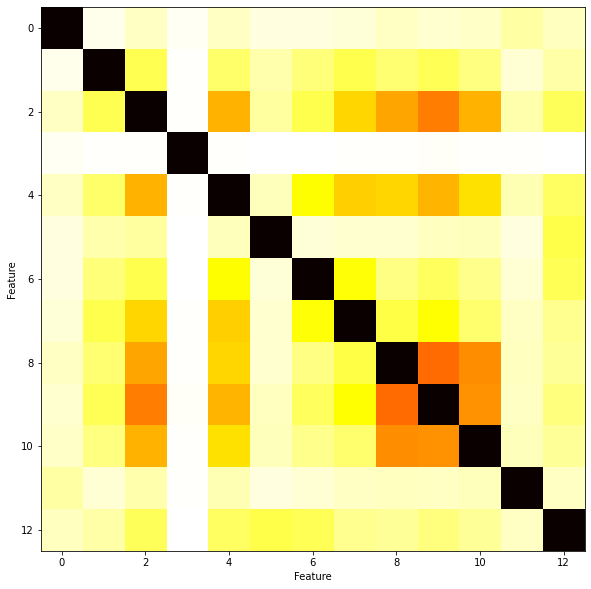
\includegraphics[width=0.4\textwidth]{miscoding_matrix.png}
\caption{Regular Miscoding Matrix.}
\label{figure:miscoding_matrix}
\end{figure}

The minimum value of $0.52$ is obtained with the pair $(8, 9)$ that correspond to the features "index of accessibility to radial highways" and "full-value property-tax rate per \$10,000". These features are good candidates to evaluate in a predictive model, since they contain non-redundant information. The maximum value of $0.99$ is achieved with the pair $(3, 12)$ with the features "Charles River dummy variable" and "\% lower status of the population". These features contains almost the same information, and so, including both in a model does not add nothing new, but increases the complexity of the model and the risk of over-fitting.

\end{example}

Finally, we are going to see the concept of miscoding applied to a feature and a delayed version of itself as a function of this delay, what we call auto-miscoding, and the miscoding of a feature applied over a delayed version of the target (or another feature), what we call cross-miscoding.

Auto-miscoding is intended to detect the repetitive patterns in a time series (see Section \ref{sec:intro_time_series}), for example, the presence of cycles. Auto-miscoding computes the miscoding of a time series (a vector) at time $t=0$, , with a lagged version of itself at time $t=i$, and repeat this process for a given number $n$ of lagging periods:
\[
\hat\mu(\mathbf{x}^{t=0}$, $\mathbf{x}^{t=i}) \quad i=1,\ldots,n
\]

\begin{example}
In this example we are going to study the presence of cycles in the number of passengers of a US airline. In Figure \ref{figure:air_passengers} is depicted a time series of monthly passengers from 1949 to 1960 (AirPassenger dataset, see References section bellow). As we can observe, there is a clear cycle that repeats every twelve months. We can apply the concept of auto-miscoding to validate analytically that this is the case.

\begin{figure}[h]
\centering
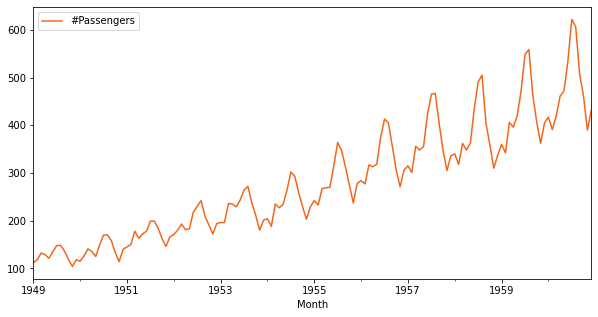
\includegraphics[width=0.6\textwidth]{airpassengers.png}
\caption{Air Passengers.}
\label{figure:air_passengers}
\end{figure}

\begin{sourcecode}
{\scriptsize \begin{verbatim}
from fastautoml.fastautoml import Miscoding

data = pd.read_csv("data/AirPassengers.csv", index_col=["Month"], parse_dates=True)
X = np.array(data["#Passengers"]).reshape(-1, 1)

miscoding = Miscoding()
miscoding.fit(X, y=None)
mscd = miscoding.auto_miscoding(attribute=0, max_lag=36, mode='adjusted')
\end{verbatim}}
\end{sourcecode}

As we can see in Figure \ref{figure:auto-miscoding} there is a peak on the value of auto-miscoding every twelve months. That means that the distance of the time series is minimal with respect to a yearly lagged versions of itself.

\begin{figure}[h]
\centering
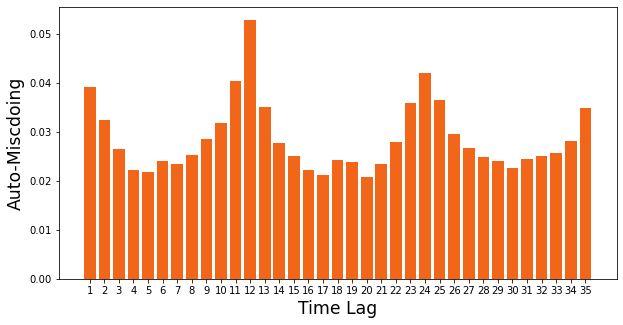
\includegraphics[width=0.6\textwidth]{auto-miscoding.png}
\caption{Auto-miscoding of Air Passengers.}
\label{figure:auto-miscoding}
\end{figure}

\end{example}

Cross-miscoding computes the inter-relation between a time series and a lagged version of a second time series. The objective is to detect if the first time series has a temporal predictive power over the second. Given a candidate predictive feature $\mathbf{x}$ and a target $\mathbf{y}$ (or a second feature), cross-miscoding computes the following quantity:
\[
\hat\mu(\mathbf{x}^{t=0}, \mathbf{y}^{t=i}) \quad i=1,\ldots,n
\]

\begin{example}
We are interested to determine if it possible to predict the energy consumption of the appliances of a house. The data set to study (appliances energy prediction dataset, see References below) is composed by the temperature and humidity conditions measured in the different rooms of the house every ten minutes, and the energy consumption of the appliances. The dataset also includes some information about the current weather, from a nearby weather station.

For every feature we will compute the optimal lag at which the features has the best prediction capabilities:

\begin{sourcecode}
{\scriptsize \begin{verbatim}
from fastautoml.fastautoml import Miscoding

X = pd.read_csv("../data/energydata_complete.csv", parse_dates=["date"], index_col="date")
y = X["Appliances"]
X = X.drop(["Appliances", "lights"], axis=1)

miscoding = Miscoding()
miscoding.fit(X, y)

best_lag  = list()
for i in np.arange(X.shape[1]):
    mscd = miscoding.cross_miscoding(attribute1=i, min_lag=1, max_lag=30)
    best_lag.append(np.where(mscd == np.max(mscd))[0][0] + 1)
\end{verbatim}}
\end{sourcecode}

In Figure \ref{figure:cross-miscoding} we can see a plot of the results. As we can observe, in general, for the in-house measurements we should use small lag values. However, in case of the weather conditions, bigger lags provide better results.

\begin{figure}[h]
\centering
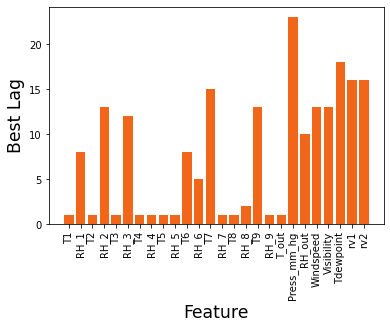
\includegraphics[width=0.6\textwidth]{cross_miscoding_lag.png}
\caption{Cross Miscoding Lag}
\label{figure:cross-miscoding}
\end{figure}

\end{example}

\begin{remark}
The approximation to the concept of miscoding introduced in this chapter estimates the quality of individual features as predictors of a target value, and the quality of the training dataset as a whole. However, the current approximation does not take into account the existing redundancy among the features themselves. For example, it might happen that two features $\mathbf{x}_i$ and $\mathbf{x}_j$ have very low miscoding with respect to the target variable $\mathbf{y}$, but at the same time they are redundant, in the sense that they contain almost the same information. It is still an open question how to extend the concept of miscoding to take into account feature redundancy, in such a way that it is close to the theoretical definition, it can be computed efficiently, and it does not require a huge number of samples.
\end{remark}

%
% Section: Inaccuracy
%

\section{Inaccuracy}
\label{sec:machine_learning_inaccuracy}

In Section \ref{sec:inaccuracy:inaccuracy} we defined the inaccuracy of a description $d \in \mathcal{D}$ for a representation $r \in \mathcal{R}$ as the normalized information distance between the representation $r$ and the string $\Gamma(d)$ printed out by a universal Turing machine when given the description as input:
\[
\iota(d, r) = \frac{ \max\{ K \left(r \mid \Gamma(d) \right), K \left( \Gamma(d) \mid r \right) \} } { \max\{ K(r), K \left(\Gamma(d) \right) \} }
\]

Inaccuracy, being based in Kolmogorov complexity, is not computable for the general case, and so, it has to be approximated in practice. In this section we are going to see how this concept can be estimated in case of a model trained using a dataset. The approach will be similar to the one used in case of miscoding (see Section \ref{sec:approx-miscoding} for more information).




{\color{red} TODO: This definition correspond to the discriminative case. Introduce the generative case as well.}

\begin{definition}
Let $\mathbb{X}$ be a dataset, $\mathbf{y}$ a response variable, $m$ a model, and $\mathbf{\hat{y}} = m(\mathbb{X})$ the predicted values by $m$ given $\mathbb{X}$. We define the \emph{inaccuracy}\index{Inaccuracy} of the model $m$ for the target values $\mathbf{y}$, denoted by $\hat\iota(\mathbf{\hat{y}}, \mathbf{y})$, as:
\[
\hat\iota(\mathbf{\hat{y}}, \mathbf{y}) = \frac{ \hat{K}_C(\mathbf{\hat{y}}, \mathbf{y}) - \min\{ \hat{K}_C(\mathbf{\hat{y}}), \hat{K}_C(\mathbf{y}) \} } { \max\{ \hat{K}_C(\mathbf{\hat{y}}), \hat{K}_C(\mathbf{y}) \} }
\]\end{definition}

Intuitively, the quantity $\hat\iota(\mathbf{\hat{y}}, \mathbf{y})$ is a measure of how far are the predicted values from real values. The lower this quantity, the better is the quality of $m$ as a predictor for $\mathbf{y}$. With our new inaccuracy metric we are measuring not only how difficult is to reconstruct the original target vector $\mathbf{y}$ given the predicted values $\mathbf{\hat{y}}$, but also how much additional information $\mathbf{\hat{y}}$ contains that is not related to $\mathbf{y}$, being the latter a novelty with respect to other metrics used in machine learning to measure the accuracy of a model.

\begin{example}
\label{ex:machine_learning:inaccuracy:inaccuracy_DT}
Inaccuracy, according to the minimum nescience principle, is given by the normalized compression distance between the actual targets $\mathbf{y}$ and the predicted targets $\mathbf{\hat{y}}$ by the model. In the following example we are going to compare the behavior of our new inaccuracy metric with a classical score metric. The experiment will be based on the MNIST\index{MNIST} dataset (hand written digits recognition) provided by scikit-learn.

\begin{sourcecode}
{\scriptsize \begin{verbatim}
from fastautoml.fastautoml import Inaccuracy
from sklearn.datasets import load_digits

X, y = load_digits(return_X_y=True)

inacc = Inaccuracy()
inacc.fit(X, y)
\end{verbatim}}
\end{sourcecode}

For this example we will train a decision tree classifier up to a pre-determined tree depth of $i$, where $i$ goes from $1$ to $20$.

\begin{sourcecode}
{\scriptsize \begin{verbatim}
from sklearn.tree import DecisionTreeClassifier

scores       = list()
inaccuracies = list()

for i in range(20):
    
    tree = DecisionTreeClassifier(max_depth=i, random_state=42)
    tree.fit(X, y)
    
    scores.append(1 - tree.score(X, y))
    inaccuracies.append(inacc.inaccuracy_model(tree))
\end{verbatim}}
\end{sourcecode}

We are interested to compare the behavior of score (actually we are comparing against one minus score) and inaccuracy metrics. As we can see in Figure \ref{figure:machine_learning:inaccuracy:inaccuracy_DT}, both metrics present a similar behavior, having inaccuracy a larger value, due to a stronger emphasis in incorrectly predicted values.

\begin{figure}[h]
\centering
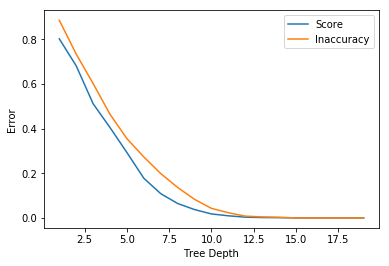
\includegraphics[width=0.6\textwidth]{inaccuracy_DT.png}
\caption{Inaccuracy vs. Score of Decison Trees}
\label{figure:machine_learning:inaccuracy:inaccuracy_DT}
\end{figure}

\end{example}

In Example \ref{ex:machine_learning:inaccuracy:inaccuracy_DT} we have seen that the deeper the tree, the smaller is the training error. Of course, the higher the value of $i$, the higher the risk of overfitting\index{Overfitting} the data. However, in case of inaccuracy we are not interested in avoiding overfitting, since overfitting is controlled by the metric of surfeit (see Section \ref{sec:machine_learning:surfeit}).

We can see inaccuracy as the effort, measured as the length of a computer program, required to fix the predictions made by a model. In this sense, according to the minimum nescience principle, it is not the same a model that makes one hundred times the same error than a model that makes one hundred different errors, since it should be easier to fix the former than the later (see Example \ref{ex:machine_learning:inaccuracy:one_hundred_errors}).

\begin{example}
\label{ex:machine_learning:inaccuracy:one_hundred_errors}
In this example we are going to use again a decision tree classifier, but this time it will be trained with the hyperparameter minimum number of samples per leaf node set to 5 (a common approach used in practice to avoid decision trees to overfit).

\begin{sourcecode}
{\scriptsize \begin{verbatim}
tree = DecisionTreeClassifier(min_samples_leaf=5)
tree.fit(X, y)
\end{verbatim}}
\end{sourcecode}

The inaccuracy of this new trained model is $0.17$, and its score $0.08$. Next we will artificially introduce one hundred errors in the dataset, simulating the case that the tree is not able to model correctly these data points. In this particular case all the errors are exactly the same.

\begin{sourcecode}
{\scriptsize \begin{verbatim}
X2 = X.copy()
y2 = y.copy()
for i in range(100):
    X2 = np.append(X2, [X[0]], axis=0)
    y2 = np.append(y2, (y[0]+1) % 10)
\end{verbatim}}
\end{sourcecode}

The inaccuracy of the decision tree, given this new dataset, has increased\footnote{Note that we had to \texttt{fit()} again the class Inaccuracy in order to use the new dataset. Normally this is not the way we use this class; instead what we should do is to fit once a dataset, and then compute the inaccuracy of different models. We are doing here in this way to demonstrate an interesting property of the concept of inaccuracy.} from $0.17$ to $0.21$.

\begin{sourcecode}
{\scriptsize \begin{verbatim}
inacc.fit(X2, y2)
inacc.inaccuracy_predictions(pred)
\end{verbatim}}
\end{sourcecode}

Score has also increased, in this case from $0.08$ to $0.13$.

\begin{sourcecode}
{\scriptsize \begin{verbatim}
1 - tree.score(X2, y2)
\end{verbatim}}
\end{sourcecode}

Finally, we are going to repeat exactly the same experiment, but this time instead of adding one hundred times the same error, adding one hundred different errors.

\begin{sourcecode}
{\scriptsize \begin{verbatim}
X3 = X.copy()
y3 = y.copy()
for i in arange(100):
    index = np.random.randint(X.shape[0])
    X3    = np.append(X3, [X[index]], axis=0)
    y3    = np.append(y3, (y[index]+1) % 10)
\end{verbatim}}
\end{sourcecode}

In this last case the inaccuracy of the model has increased up to $0.25$, meanwhile score remained the same.
\end{example}

In line with Example \ref{ex:machine_learning:inaccuracy:one_hundred_errors}, an extreme case would be a model for a target binary variable (True and False) that always fails with its predictions, that is, if the value of the target is True, the model will predict False, and if it is False, it will predict True. The classical evaluation metrics would say that this model is the worst possible model, but our inaccuracy would claim that the model is perfect. We might be wondering what it is the value of a model that always fails to predict the correct target. But if we are the managers of an edge fund investing in the stock market\index{Stock market}, we will very happy to pay a huge amount of money for a model that predicts that the shares of IBM will go down whenever they go up, and the other way around.

In case of having a highly unbalanced dataset\index{Unbalance dataset}, that is, when some categories have a lot of more training data than others, the classical score metric can provide a misleading result, since a good score does not necessarily mean a good model, it might happen that the model is simply properly classifying the samples of the category with the higher number of training samples, and misclassifying the others. In practice, we solve this problem by using metrics specifically designed to deal with unbalanced datasets. In case of the new metric of inaccuracy, as Example \ref{ex:machine_learning:inaccuracy:unbalanced_dataset} shows, a model that can not properly classify one of the categories is considered a bad model, even if this category has only a few points in the training dataset.

\begin{example}
\label{ex:machine_learning:inaccuracy:unbalanced_dataset}
For this example, we will create a synthetic dataset using the \texttt{make\_classification} utility of scikit-learn, with two classes in which one of then has 95\% of the samples, and the other 5\%.

\begin{sourcecode}
{\scriptsize \begin{verbatim}
from sklearn.datasets import make_classification

depth = list()
score = list()
inacc = list()

inaccuracy = Inaccuracy()

for i in np.arange(1, 100):
                    
    X, y = make_classification(n_samples=1000, n_features=2,
                               n_informative=2, n_redundant=0,
                               class_sep=2, flip_y=0, weights=[0.95,0.05])

    inaccuracy.fit(X, y)
        
    tree = DecisionTreeClassifier(min_samples_leaf=i)
    tree.fit(X, y)

    depth.append(i)        
    score.append(1 - tree.score(X, y))
    inacc.append(inaccuracy.inaccuracy_model(tree))
\end{verbatim}}
\end{sourcecode}

The experiment consists in training a decision tree classifier with a minimum number of samples per leaf of $i$, where $i$ goes from 1 to 100. In Figure \ref{figure:machine_learning:inaccuracy:inaccuracy_DT2} we can see the behavior of inaccuracy and score. In case of large values of $i$, the score metric tell us that no more than a 5\% of the samples is misclassified, however, the inaccuracy says that even if the total number of misclassified points is low, the inaccuracy of the model is very bad.

\begin{figure}[h]
\centering
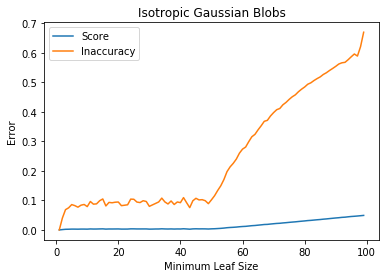
\includegraphics[width=0.6\textwidth]{inaccuracy_DT2.png}
\caption{Inaccuracy of Decision Tree.}
\label{figure:machine_learning:inaccuracy:inaccuracy_DT2}
\end{figure}

\end{example}





%
% Section: Surfeit
%

\section{Surfeit}
\label{sec:machine_learning_surfeit}

In Section \ref{sec:Definition_redundancy} we defined the surfeit of the model $m \in \mathcal{M}$ for the representation $r \in \mathcal{R}$ as:
\[
\sigma (m, r) = 1 - \frac{K(r)}{l(m)}
\]
Since the length $K(r)$ of shortest possible model for the representation $r$ is in general unknown, we have to approximate this concept in practice. In case of having a training dataset $\mathbb{X}$ and a target variable $\mathbf{y}$, we can approximate the surfeit of a model $m$ for the representation $\mathbf{y}$ by means of computing:
\[
\hat\sigma(m, y) = 1 - \frac{\hat{K}_C(\mathbf{y})}{l(m)}
\]
Where $\hat{K}_C(\mathbf{y})$ is the length of the compressed version of the of the vector $\mathbf{y}$ using as compressor a minimal length code $C$, computed given the relative frequencies of the values observed in $\mathbf{y}$ (see Section \ref{sec:approx-miscoding}).

\begin{definition}
Let $\mathbf{y}$ be a response variable, $\mathbb{X}$ a dataset composed by $p$ features and $n$ samples. We define the surfeit of the model $m \in \mathcal{M}$ as a representation of $\mathbf{y}$, denoted by $\hat\sigma(m, \mathbf{y})$, as:
\[
\hat\sigma(m, \mathbf{y}) = 1 - \frac{\hat{K}_C(\mathbf{y})}{l(m)}
\]
\end{definition}

The definition of surfeit requires a method of encoding the models as a string of symbols, so we can compute their length. Ideally, we should use as encodings Turing machines, and agree upon an universal Turing machine to interpret those models. However, that would make very difficult to add new models to the nescience library. Instead, we have used for the encoding of models a simplified version of the Python language, where not all the constructions are allowed, and we do not allow the use of libraries.

Surfeit is a metric that can help us to avoid overfitted models. The higher is the surfeit of a model, the higher is the probability that the model is an overfit of the training dataset, as Example \ref{ex:surfeit_overfit} shows.

\begin{example}
\label{ex:surfeit_overfit}
In this example we are going to generate a dataset composed by $900$ samples of a sinusoidal curve, and we will fit the data using a $n$ degree polynomial, where $n$ goes form $1$ to $15$.

\begin{sourcecode}
{\scriptsize \begin{verbatim}
from sklearn.linear_model import LinearRegression
from sklearn.preprocessing import PolynomialFeatures

from Nescience.Nescience import Surfeit
from Nescience.Nescience import Inaccuracy

n_samples = 900
degrees = np.arange(1, 15)

X = np.sort(np.random.rand(n_samples) * 3)
y = np.cos(1.5 * np.pi * X)

linacc   = list()
lsurfeit = list()

for i in degrees:
        
    poly = PolynomialFeatures(degree=i, include_bias=False)
    newX = poly.fit_transform(X[:, np.newaxis])
    
    linear_regression = LinearRegression()
    linear_regression.fit(newX, y)

    inacc.fit(newX, y)
    inaccuracy = inacc.inaccuracy_model(linear_regression)
    
    sft.fit(newX, y)
    surfeit = sft.surfeit_model(linear_regression)
    
    linacc.append(inaccuracy)
    lsurfeit.append(surfeit)
\end{verbatim}}
\end{sourcecode}

In figure \ref{figure:surfeit_vs_inaccuracy} we can see the results of this experiment. As it was expected, the higher the degree of the polynomial, the smaller is the error of the model. However, at the same time we see that the higher the polynomial, the higher the surfeit of the model. The ideal model is that one that has a low inaccuracy and a low surfeit.

\begin{figure}[h]
\centering
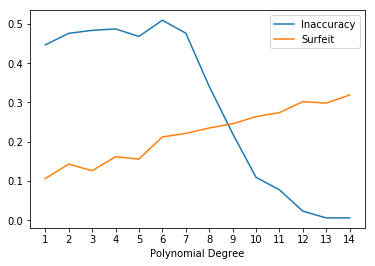
\includegraphics[width=0.6\textwidth]{surfeit_vs_inaccuracy.png}
\caption{Surfeit vs Inaccuracy}
\label{figure:surfeit_vs_inaccuracy}
\end{figure}

\end{example}

Another advantage of the concept of surfeit is that it allows us to compare and decide between models that belong to different families. For example, in case of models having the same accuracy, shall we prefer a decision tree over a neural network, or a naive Bayes classifier over a support vector machine? Next example shows how we can decide about those questions.

\begin{example}
\label{ex:dt_vs_nn}

In this example we are going to compare a decision tree with a neural network. We will use a synthetic dataset composed by two isotropic Gaussian blobs, and we will train our models to split them apart. In the first part of the example we will use a standard deviation of $1$ and only two dimensions, so the two clusters are easy to classify (see figure on Table \ref{tab:isotropic_gaussian_blobs}, left side).

\begin{table}
\begin{center}

\begin{tabular}{ c c }

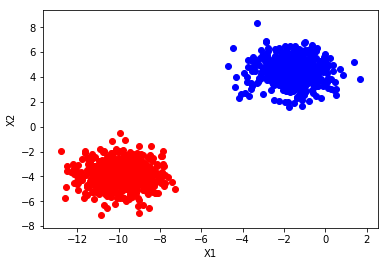
\includegraphics[scale=0.4]{blobs_easy_split} & 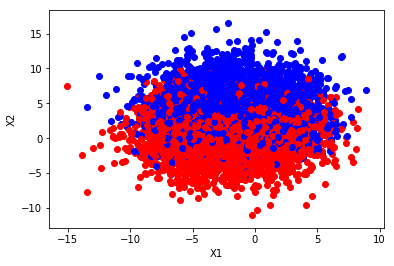
\includegraphics[scale=0.4]{blobs_difficult_split}

\end{tabular}
\end{center}
\caption{\label{tab:isotropic_gaussian_blobs}Isotropic Gaussian blobs.}
\end{table}

% \raisebox{.4\height}{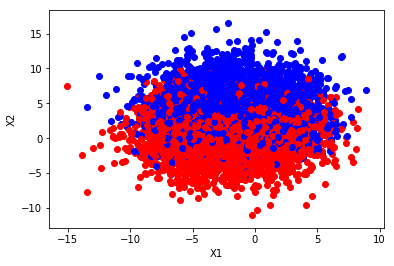
\includegraphics[scale=0.4]{blobs_difficult_split}}

\begin{sourcecode}
{\scriptsize \begin{verbatim}
from sklearn.tree import DecisionTreeClassifier
from sklearn.neural_network import MLPClassifier
from Nescience.Nescience import Surfeit
from Nescience.Nescience import Inaccuracy
from sklearn.datasets.samples_generator import make_blobs

X, y = make_blobs(n_samples=1000, centers=2, n_features=2, cluster_std=1)

tree = DecisionTreeClassifier()
tree.fit(X, y)
tree.score(X, y)

nn = MLPClassifier()
nn.fit(X, y)
nn.score(X, y)

sft = Surfeit()
sft.fit(X, y)

sft.surfeit_model(tree)
sft.surfeit_model(nn)

\end{verbatim}}
\end{sourcecode}

If we ran the above code we will see that both models have exactly the same accuracy of $1$, that is, they are perfect classifiers. However the surfeit of the decision tree is $0.25$, meanwhile the surfeit of the neural network is $0.73$. In this particular case we should prefer the decision tree over the neural network.

If we perform the same experiment using a standard deviation of $3$, so two clusters that are more difficult to split (see Table \ref{tab:isotropic_gaussian_blobs}, right side), the situation will change.

\begin{sourcecode}
{\scriptsize \begin{verbatim}
X, y = make_blobs(n_samples=10000, centers=2, n_features=8, cluster_std=3)
\end{verbatim}}
\end{sourcecode}

In this second case, again, both models have the same accuracy (we have increased the number of samples, and the number of dimensions, so the models can still perform a perfect classification), but the surfeit of the decision tree has increased to $0.82$, and the surfeit of the neural network is almost the same, $0.76$. For this second dataset we should prefer the neural network over the decision tree.

\end{example}

In example \ref{ex:dt_vs_nn} we have assumed that both models, decision tree and neural networks, have the same accuracy. When this is not the case, when the models do not have the same accuracy, we have to apply to the concept of nescience in order to decide between them. 

\begin{remark}
{\color{red} TODO: Mention the problem of the stability of the signal.}
\end{remark}

%
% Section: Nescience
%

\section{Nescience}
\label{sec:machine_learning_nescience}

In Chapter \ref{chap:Nescience} we defined the concept of nescience as the solution to a non-linear multi-objective optimization problem, where we had to minimize the miscoding, inaccuracy and surfeit of representations and models. The solution to this problem is, in general, not unique, in the sense that we can find multiple pairs of representations and models that have the property that we can not improve one of these quantities without degrading the others (Pareto optimality). However, in practice, we expect that a machine learning library should provide a single solution when training a model over a dataset. In order to provide this unique solution, we have to resort to a utility function that selects one from the available solutions. The nescience library provide different alternatives of utility functions, being the default one the arithmetic mean the tree metrics.

\begin{remark}
The nescience library implements the following utility functions to approximate the concept of nescience, that is, to compute $\hat\nu\left(\mathbb{Z}, m, \mathbf{y} \right)$:

\begin{itemize}
\item Euclid distance: $\left( \hat\mu(\mathbb{Z}, \mathbf{y})^2 + \hat\iota(\hat{y}, \mathbf{y})^2  + \hat\sigma(m, \mathbf{y})^2 \right)^{1/2}$
\item Arithmetic mean: $\frac{\hat\mu(\mathbb{Z}, \mathbf{y}) + \hat\iota(\hat{y}, \mathbf{y}) + \hat\sigma(m, \mathbf{y})}{3}$
\item Geometric mean: $\left( \hat\mu(\mathbb{Z}, \mathbf{y}) \times \hat\iota(\hat{y}, \mathbf{y}) \times \hat\sigma(m, \mathbf{y}) \right)^{1/3}$
\item Product: $\hat\mu(\mathbb{Z}, \mathbf{y}) \times \hat\iota(\hat{y}, \mathbf{y}) \times \hat\sigma(m, \mathbf{y})$
\item Addition: $\hat\mu(\mathbb{Z}, \mathbf{y}) + \hat\iota(\hat{y}, \mathbf{y}) + \hat\sigma(m, \mathbf{y})$
\item Weighted mean: $w_\mu \hat\mu(\mathbb{Z}, \mathbf{y}) + w_\iota \hat\iota(\hat{y}, \mathbf{y}) + w_\sigma \hat\sigma(m, \mathbf{y})$
\item Harmonic mean: $\frac{3}{ \hat\mu(\mathbb{Z}, \mathbf{y})^{-1} + \hat\iota(\hat{y}, \mathbf{y})^{-1} + \hat\sigma(m, \mathbf{y})^{-1} }$
\end{itemize}

Euclid distance and addition have the drawback that they produce nescience values greater than one, something that it is against our theory. Geometric mean, product and harmonic mean have the problem that the nescience is zero, or not defined, if one of the three metrics (miscoding, inaccuracy or surfeit) is zero. And the weighted mean introduce three new hyperparameters that have to be optimized. It is still an open question which one is the best utility function to compute the nescience of a dataset and a model.
\end{remark}

Example \ref{ex:nescience_decisiontree} shows how we can use the \texttt{nescience} library to compute the nescience of a dataset and a model.

\begin{example}
\label{ex:nescience_decisiontree}

This example shows how to compute in practice the nescience of a dataset and a model. In particular, we are going to compute the nescience of a decision tree classifier applied over the dataset digits (MNIST hand written digits classification problem) included in the \texttt{sklearn} library.

\begin{sourcecode}
{\scriptsize \begin{verbatim}
from sklearn.tree import DecisionTreeClassifier
from sklearn.datasets import load_digits
from Nescience.Nescience import Nescience

data = load_digits()

tree = DecisionTreeClassifier()
tree.fit(data.data, data.target)
tree.score(data.data, data.target
[ ] 1

nescience = Nescience()
nescience.fit(data.data, data.target)

nescience.nescience(tree)
[ ] 0.5895603819965907
\end{verbatim}}
\end{sourcecode}

The score of the decision tree model is $1$, meaning that all the samples have been properly classified. Of course, what happened is that the decision tree is overfitting the dataset. In order to avoid this kind of problems we usually split the data in separate training and testing subsets, or we perform a more advanced cross-validation. However, if we compute the nescience, we will get a value of $0.59$, rising the flag that something is wrong with the model or the training dataset.

\end{example}

In Example \ref{ex:nescience_decisiontree} we have shown that one of the advantages of the concept of nescience is that we can evaluate the quality of a model without applying computationally expensive procedures like cross-validation, and without requiring to save part of the data as a test subset. Another advantage of the metric nescience is that it allows us to decide between competing models from different families of models, as it is shown in Example \ref{ex:nescience_comparison}.

\begin{example}
\label{ex:nescience_comparison}

In this example we are going to compare two models from two different families of models: decision trees and neural networks. Both models will be trained with the breast cancer dataset provided by the \texttt{sklearn} library.

\begin{sourcecode}
{\scriptsize \begin{verbatim}
from sklearn.tree import DecisionTreeClassifier
from sklearn.neural_network import MLPClassifier
from sklearn.datasets import load_breast_cancer
from Nescience.Nescience import Nescience

data = load_breast_cancer()
X = data.data
y = data.target

tree = DecisionTreeClassifier(max_depth=3)
tree.fit(X, y)
tree.score(X, y)
[ ] 0.9789103690685413

nescience = Nescience()
nescience.fit(X, y)
nescience.nescience(tree)
[ ] 0.5945936419010083

nn = MLPClassifier()
nn.fit(X, y)
nn.score(X, y)
[ ] 0.9261862917398945

nescience.nescience(nn)
[ ] 0.7860523786210711
\end{verbatim}}
\end{sourcecode}

Both models have a similar score. In this case, not only the decision tree provide a better score, but also, the nescience is much lower than in case of the multi-layer perceptron, and so, we should prefer the former over the later.

\end{example}

Nescience is a metric that can be used to optimize the hyperparameters that define a (parametric) family of models. The advantage of nescience is that we can use a greeedy approach to select the best value for an hypeparameter, saving a lot of computational time and resources during the search. That is, if we have a model controlled by an hyperparameter such that the higher the value the better the score, we should select that value in which the nescience stops decreasing and starts to increase, since this is the point in which we are not longer learning anything new from that dataset (see Example \ref{ex:nescence_hyperparameter}).

\begin{example}
\label{ex:nescence_hyperparameter}

For this example we will use again a decision tree classifier with the breast cancer dataset. We will train $10$ different trees, setting the hyperparameter \texttt{max\_depth} with values from $1$ to $10$. The \texttt{max\_depth} hyperparameter controls how deep we allow the tree to grow in order to classify the samples of the dataset. The deeper the tree the higher the score of the model, but also, the higher the risk of overfitting the training data. For each tree we will compute the nescience of the model, and we will compare it with a cross validation score. The results are shown in Figure \ref{figure:nescience_cancer}. As we can see in the figure, both, nescience and cross validation score, decrease are we increase the depth of the tree, until we reach a point in which it starts to increase. This inflection point is where the model begins to overfit the data. The nescience library suggests to use a tree with a maximum depth of $7$, meanwhile with the cross validation we got an optimal level of 6.

\begin{figure}[h]
\centering
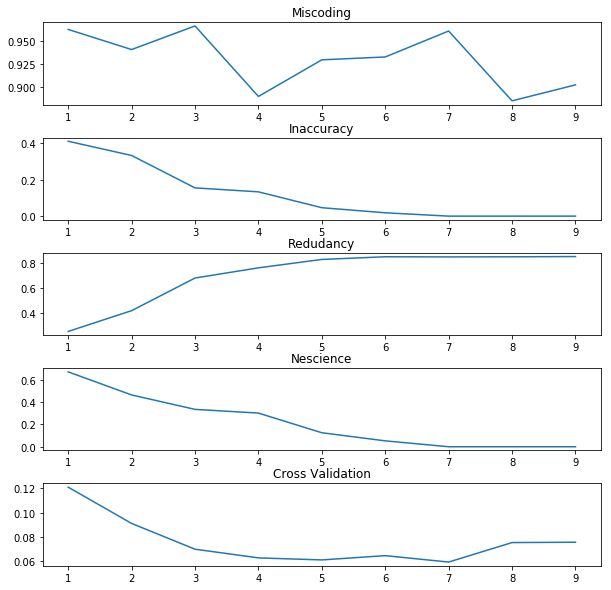
\includegraphics[width=0.6\textwidth]{nescience_cancer.png}
\caption{Evolution of Nescience with Tree Depth.}
\label{figure:nescience_cancer}
\end{figure}

\end{example}

It is interesting to note the behavior of the three metrics that define the concept of nescience in Figure \ref{figure:nescience_cancer}. As it is expected the the deeper the tree the smaller is the inaccuracy of the model and the higher the surfeit. However, in case of miscoding, we have a sort of random evolution. This behavior is due to the fact that each candidate tree uses a different subset of features at the decision nodes. I would be very nice to have an decision tree building algorithm that takes into account miscoding in order to decide the best features for new branches. Such an algorithm is described in Section \ref{sec:decision_trees}.

Finally, we are going to see how to use nescience in case of hyperparameter searches where we cannot apply a greedy approach, for example when the search is performed over a collection of (usually conflicting) hyperparameters. Hyperparameter search is a computationally expensive approach, since the number of possible combinations to test could be very large. Moreover, if for each candidate set we have to cross-validate the result, the search becomes prohibitive. As we have seen, nescience do not requires the use of crossvalidation to detect a situation of overfiting, and so, it can significantly speed up the process of searching for optimal hyperparameters. In Example \ref{ex:hyper_search} it is show how we can do that with the \texttt{nescience} library.

\begin{example}
\label{ex:hyper_search}

In this example we are going to see how we can use the \texttt{nescience} library to find the optimal hyperparameters for a model using a grid search. In particular, we are going to select the best hyperparameters for a multilayer perceptron classifer, including the number of hidden layers, and the size of those layers (what it is called Neural Architecture Search). The procedure will be demonstrated using the \texttt{digits} dataset.

\begin{sourcecode}
{\scriptsize \begin{verbatim}
from Nescience.Nescience import Nescience
from sklearn.neural_network import MLPClassifier
from sklearn.model_selection import GridSearchCV
from sklearn.metrics import classification_report
from sklearn.model_selection import train_test_split
\end{verbatim}}
\end{sourcecode}

First of all we have to provide a custom loss function based on the concept of nescience to be integrated with the search procedure. The next code shows how to implement such a function.

\begin{sourcecode}
{\scriptsize \begin{verbatim}
def my_custom_loss_func(estimator, X, y):
    
    nsc = Nescience()
    nsc.fit(X, y)
    nescience = nsc.nescience(estimator)
    
    # scikit-learn expect that higher numbers are better
    score = -nescience
    
    return score
\end{verbatim}}
\end{sourcecode}

Second, we have to define the grid of hyperparameters over which we are going to do the search. The larger the grid, the better the result, but also, the more computer time is required to evaluate all possible combinations.

\begin{sourcecode}
{\scriptsize \begin{verbatim}
parameters = {'solver': ['lbfgs'],
              'max_iter': [1000, 1500, 2000 ], 
              'alpha': 10.0 ** -np.arange(1, 10, 3),
              'hidden_layer_sizes':[(60,), (100,), (60, 60,), (100, 100,), 
                                    (60, 60, 60,), (100, 100, 100,)]}
\end{verbatim}}
\end{sourcecode}

Next code show how to do a classical grid search using the score of the models. The search will be evaluated using a train/test split of the dataset.
 
\begin{sourcecode}
{\scriptsize \begin{verbatim}
clf_std = GridSearchCV(estimator=MLPClassifier(), param_grid=parameters,
                       cv=3, iid=True, n_jobs=-1)
clf_std.fit(X_train, y_train)
clf_std.best_params_

[] {'alpha': 0.1,
[]  'hidden_layer_sizes': (100,),
[]  'max_iter': 1000,
[]  'solver': 'lbfgs'}

y_true, y_pred = y_test, clf_std.predict(X_test)
print(classification_report(y_true, y_pred))

[] precision    recall  f1-score   support
[] avg / total       0.98      0.97      0.97       540
\end{verbatim}}
\end{sourcecode}

Next code show how to perform exactly the same search, but using the concept of nescience instead of the metric score.

\begin{sourcecode}
{\scriptsize \begin{verbatim}
clf_nsc = GridSearchCV(estimator=MLPClassifier(), param_grid=parameters,
                       cv=3, scoring=my_custom_loss_func, iid=True)
clf_nsc.fit(X_train, y_train)
clf_nsc.best_params_

{'alpha': 0.1,
 'hidden_layer_sizes': (60,),
 'max_iter': 1500,
 'solver': 'lbfgs'}

y_true, y_pred = y_test, clf_nsc.predict(X_test)
print(classification_report(y_true, y_pred))

                  precision    recall    f1-score    support
avg / total       0.98         0.98      0.98        540
\end{verbatim}}
\end{sourcecode}

As we can see, the results provided by the \texttt{nescience} library are slightly better in terms of train/test evaluations. However, what it is important is the library has opted for a smaller model (one layer of $60$ neurons instead of one layer of $100$ neurons) that provides a better result by increasing the maximum number of iterations (from $1000$ to $1500$). Nescience always select the smallest model that provides the best possible accuracy that does not overfit the training data.

\end{example}

%
% Section: Auto Classification
%

\section{Auto Machine Classification}
\label{sec:machine_learning_classification}

The nescience library also includes a module for auto-machine learning (both for classification and regression problems). The auto-machine learning module returns the model, from a collection of families of models, that provides the smalles nescience. For each family of models, the class perform a greedy search over the hyperparameters required for each family. In Appendix XX is described the detail for each family of models.

Next example shows how to apply the automachine learning tools.

\begin{example}
\label{ex:automl}

In this example we are going to see how to apply the nescience library to find the best model that describes the \texttt{digits} dataset.

\begin{sourcecode}
{\scriptsize \begin{verbatim}
from sklearn.datasets import load_digits
from sklearn.model_selection import train_test_split

from Nescience.Nescience import AutoClassifier

(X, y) = load_digits(return_X_y=True)
X_train, X_test, y_train, y_test = train_test_split(X, y, random_state=1)

model = AutoClassifier()
model.fit(X_train, y_train)

model.score(X_test, y_test)
[] 0.9622222222222222
\end{verbatim}}

If we write \texttt{type(model.model)} we will see that the library has selected a linear support vector machine as the best model for this dataset.

\end{sourcecode}
\end{example}

{\color{red} TODO: Compare with other automl tools.}

\subsection{Surfeit of Algorithms}

\subsubsection*{Decision Trees}
\label{subsec:surfeit_decision_trees}

For the representation of a tree as a string we use the following template:

\begin{sourcecode}
{\scriptsize \begin{verbatim}
def tree{[attrs]}:
    if [attr] <= [thresh]:
        return [label] || [subtree]
    else:
        return [label] || [subtree]
\end{verbatim}}
\end{sourcecode}

Where \texttt{[attrs]} is the list of attributes used, and only those used in the model,%
\footnote{If the dataset contains many attributes, listing all of them when dealing with very short models would make the length of the model's header greater than the length of the body.}  \texttt{[attr]} is a single attribute represented by the letter \texttt{X} followed by a number (e.g. \texttt{X1}), \texttt{[thresh]} is the threshold used for the split, \texttt{[label]} is one of the valid labels from the set $\mathcal{G}$, and \texttt{|| [subtree]} means that the \texttt{return} statement can be replaced by another level of \texttt{[if - else]} conditions. We could have used a much shorter description of trees by replacing word tokens with symbols, e.g., by the ternary conditional operators \texttt{?} and \texttt{:} used in modern programming languages, or by dropping the \texttt{return} statement. This would produce shorter trees, but the complexity of the models would remain the same, up to an additive constant that does not depend on the model itself. Since the harmonic mean compares relative values instead of absolute ones, this additive constant can be safely ignored.



%
% Section: Auto Regression
%

\section{Auto Machine Regression}


%
% Section: Auto Time Series
%

\section{Auto Time Series}


%
% Section: Decision Trees
%

\section{Decision Trees}
\label{sec:decision_trees}

In the last sections we have seen how to use the concepts of miscoding, inaccuracy, surfeit and nescience to evaluate the quality of datasets and models, and to automatically select a family of models and search over its hyperparameters to find the best possible description of a topic. In particular, we have studied in detail the family of binary decision trees. The procedure used in the \texttt{fastautoml} library with trees was a mix between a classical approach (a CART algorithm combined with a cost-complexity pruning), and an evaluation of candidate trees using the minimum nescience principle. In this section we are going to see a new algorithm to derive optimal trees, both for classification and regression problems, that is entirely based on the theory of nescience. The new algorithm, by design, avoids the overfitting of the training dataset without losing accuracy, it does not require the optimization of hyperparameters, thus significantly reducing the training time, and it produces much smaller and more shallow trees than traditional algorithms, facilitating the interpretability of the results.

\subsection{Algorithm Description}
\label{sub:tree_algorithm_description}

The following pseudocode shows the proposed algorithm to build a decision tree given a training dataset $(\mathbf{X}, \mathbf{y})$. The procedure is based on a breadth first traversal of trees combined with a greedy approach. It requires a function called \textsc{bestSplit()} that returns the best split of a given subset of the data into two subsets; and a second function, called \textsc{Nescience()} that provides an estimation of the nescience of the current tree. The algorithm is based on two nested loops: the external \textbf{while} loop keeps a list of the candidate nodes to grow, whereas the internal \textbf{for} loop finds the best node to grow the tree. The latter operation requires to check all possible growing options and select the one that minimizes the nescience. The exit point of the algorithm is when there are no more branches to grow. We keep track of the best nescience achieved during the building process and return the associated tree.

\begin{sourcecode}
\label{algorithm:decision_tree}
{\scriptsize \begin{verbatim}

def BUILD_TREE(data)

    nodesList <- list()
    tree <- BESTSPLIT(data)
    bestNescience <- NESCIENCE(tree)
    nodesList.append(tree)

    while not nodesList.empty()
    
        nescience <- bestNescience
        bestNode <- None
        childNode <- None
        
        for i <- 1, nodesList.length()

            node <- nodesList[i]
            
            node.child <- BESTSPLIT(node.ldata)
            tmp <- NESCIENCE(tree)
            if tmp < nescience
                nescience <- tmp
                bestNode <- i
                
            node.left <- None

        if nescience < bestNescience
            node <- nodeList[bestNode]
            bestNescience <- nescience
            nodesList.append(node.left)
                        
            if not node.left.empty() and not node.right.empty()
                nodesList.remove(bestNode)
    
    return tree
\end{verbatim}}
\end{sourcecode}

The main difference of our algorithm from other decision tree building algorithms is in the way the tree is evaluated. Instead of using only accuracy as most of the algorithms do, in addition, we take into account the complexity of the tree (surfeit) to avoid overfitting, and the quality of the subset of data used during the training process (miscoding).

\subsubsection*{Nescience}
\label{sub:tree_nescience}

The calculation of the nescience implemented in the algorithm is based on a Euclidean distance utility function (see Section \ref{sec:machine_learning_nescience}), because that one was the one that produced the best results in the tests we have performed. For the computation of miscoding and inaccuracy, we use the same techniques that the one used in the \texttt{fastautoml} library, described in Section \ref{sec:machine_learning_miscoding} and Section \ref{sec:machine_learning_inaccuracy} respectively. For the implementation of surfeit, we use the same template to describe trees that was used in the \texttt{DecisionTreeClassifier} of the \texttt{AutoClassifier} class, and that was described in Section \ref{subsec:surfeit_decision_trees}. The only difference is that we also allow equalities in the nodes (\texttt{if [attr] = [thresh]}), something not supported by the \texttt{DecisionTreeClassifier} algorithm of the \texttt{scikit-learn} library.

The generic problem of the instability of inaccuracy due to very short models, also applies to this algorithm (see Section \ref{sec:machine_learning_surfeit}), and the particular problem of the algorithms to build decision trees, in which the best local split might not be that one that minimizes the error (see Section \ref{sec:sec:machine_learning_classification}) is also relevant in this case.

The concept of nescience is used in two different ways in our algorithm. For every iteration of the \texttt{for} loop we have to decide which one of the candidate branches of the tree we should develop. Recall that the order in which we develop the branches is important, since it might happens that one branch does not get develped because that would mean increase the sufeit without a sufficiently large decrease of the inaccuracy. The second place is a the end of the \texttt{while} loop, we we keep trac of the nescience of the different building steps, to decide at the end of the algorithm with wich tree we return.

We treat regression problems as classification problems in which we discretizes the continuous target variable $\mathbf{y}$ into $n$ intervals given the number of samples, and using a uniform discretization (see Section \label{sec:codes_continuous_data}). Once the target variable has been discretized, we train a regular classification tree.

\subsubsection*{Splitting Criteria}
\label{sub:tree_splitting_criteria}

Given a subset $\mathbf{Q} \subseteq \mathbf{X}$ we have to find an split for $\mathbf{Q}$ such that the values of $\textbf{y}$ are grouped together. Recall that a split is a pair $\theta = (j,w)$, were $1 \leq j \leq p$ is a feature index and $w$ is the partition point (see Section \ref{subsec:learning_decision_trees}). A split divides the set $\mathbf{Q}$ into two disjoint subsets $\mathbf{Q}_l$ and $\mathbf{Q}_r = \mathbf{Q} \backslash \mathbf{Q}_l$. In case of a continuous variable we have that $\mathbf{Q}_l = \{\mathbf{x}_i \in \mathbf{Q} : x_{ij} \leq w\}$, and if the feature is categorical we define $\mathbf{Q}_l = \{\mathbf{x}_i \in \mathbf{Q} : x_{ij} = w\}$\footnote{Ideally, for the categorical case, instead of a single feature $w$ we should search over all the elements of the power set of the set of features $\mathcal{P} \{1, 2, \ldots, p \}$. Unfortunately, that would imply to check $2^p$ cases, something that is time-expensive from the computational point of view.}.

In Section \ref{subsec:learning_decision_trees} we saw that a common splitting criteria used in practice is to minimize the weighted entropy $\tilde{H}$ of the subsets $\mathbf{Q}_l$ and $\mathbf{Q}_r$, that is, to find an split that it is minimal $\theta^\star = \argmin_\theta \tilde{H}(\mathbf{Q},\theta)$. More explicitly, if $\mathbf{y}$ is a target vector taking values from a set of $k$ labels $\mathcal{G} = \{g_1, \ldots, g_k \}$ (either because is a categorical target or a continuous target that has been discretized into $k$ intervals), and denoting the subsets of $\mathbf{y}$ as $\mathbf{y}^l = \{y_i : \mathbf{x}_i \in \mathbf{Q}_l \}$ and $\mathbf{y}^r = \{y_i : \mathbf{x}_i \in \mathbf{Q}_r \}$, and $n_l$ and $n_r$ are the number of elements of $\mathbf{y}^l$ and $\mathbf{y}^r$ respectively, we have that
\begin{multline}
\tilde{H}(\mathbf{Q},\theta) = \frac{n_l}{n} \left( - \sum_{i=1}^k \frac{ \sum_{j=1}^{n_l} I(y^l_j = g_i)} {n_l} \log_2{ \frac{ \sum_{j=1}^{n_l} I(y^l_j = g_i)} {n_l} } \right) \\
+ \frac{n_r}{n} \left( - \sum_{i=1}^k \frac{ \sum_{j=1}^{n_r} I(y^r_j = g_i)} {n_r} \log_2{ \frac{ \sum_{j=1}^{n_r} I(y^r_j = g_i)} {n_r} } \right)
\end{multline}

In our nescience based decision tree algorithm, the splitting criteria is to minimize the total length of encoding the subsets $\mathbf{Q}_l$ and $\mathbf{Q}_r$ using optimal codes. We have to find the optimal split $ \theta^\star = \argmin_\theta \hat{K}_C(\mathbf{Q} \mid \theta) = \argmin_\theta \{ \hat{K}_{C_l}(\mathbf{Q}_l) + \hat{K}_{C_r}(\mathbf{Q}_r) \}$ where $C_l$ and $C_r$ are the optimal codes given the relative frequencies of the observed values of $\mathbf{y}^l$ and $\mathbf{y}^r$ respectively. The quantity $\hat{K}_C(\mathbf{Q} \mid \theta)$ is computed as:
\[
\hat{K}_C(\mathbf{Q} \mid \theta) = \hat{K}_{C_l}(\mathbf{Q}_l) + \hat{K}_{C_r}(\mathbf{Q}_r) = - \sum_{i=1}^k \log_2{ \frac{ \sum_{j=1}^{n_l} I(y^l_j = g_i)} {n_l} } - \sum_{i=1}^k \log_2{ \frac{ \sum_{j=1}^{n_r} I(y^r_j = g_i)} {n_r} }
\]
I this particular case (if we use as compression algorithm a code with optimal lengths, and continuous variables have been discretized) it turns out that both expressions are equivalent given the following relation:
\[
\tilde{H}(\mathbf{Q},\theta) = \frac{1}{n} \hat{K}_C(\mathbf{Q} \mid \theta)
\]
We prefer to talk of encoding length instead of weighted entropy because it has an easier interpretation in the context of the theory of nescience.

\begin{remark}
Strictly speaking, if we want to implement a decision trees search algorithm fully compliant with the minimum nescience principle, instead of using a total length encoding as splitting criteria, we should had computed the nescience at each split and select that one that makes it minimal. However, early experiments have shown that at local level it works better to group the values of $y$ than to reduce the nescience. Further research is required to confirm and explain this point.
\end{remark}

\subsubsection*{Practical Implementation}

In the web page that accompanies this book\footnote{http://www.mathematicsunknown.com} we provide an open-source implementation of our algorithm in Python. Our software can be used together with other machine learning tools from the \texttt{scikit-learn} library, since we adhere to the their API guidelines. For example, our algorithm can be used as part of an ensemble of classifiers, like the \texttt{BaggingClassifier} meta-estimator, or the results of the classification could be cross-validated with tools like \texttt{cross\_val\_score}. As an example, to provide a model for the breast cancer dataset, we could do something like the following:

\begin{sourcecode}
{\scriptsize \begin{verbatim}
from NescienceDecisionTree import NescienceDecisionTreeClassifier
from sklearn.datasets import load_breast_cancer

data = load_breast_cancer()

model = NescienceDecisionTreeClassifier()
model.fit(data.data, data.target)
print("Score: ", model.score(data.data, data.target))
\end{verbatim}}
\end{sourcecode}

\subsection{Algorithm Evaluation}
\label{sub:algorithm_evaluation}

In this section we are going to evaluate our new algorithm, and compare its performance against the well-known algorithm CART. CART, \emph{Classification and Regression Trees}, is the de-facto standard algorithm used in the machine learning industry for the derivation of decision trees. For this particular experiment we have used the CART implementation provided by \texttt{scikit-learn}.

Figure \ref{figure:data_error_cart} shows a synthetic dataset consisting of $1000$ random points lying on a two dimensional plane, where all the points with an $X1$ attribute less than $50$ are colored blue, and the rest as red. We have artificially introduced a red point, simulating a measurement error, in the blue area. The black lines correspond to the decisions performed by CART. Since the CART algorithm will not stop until all the points have been properly classified, we have to specify an expected count condition to limit the number of splits. The figure correspond to the tree generated by CART setting the \texttt{min\_samples\_leaf} hyperparameter to $5$.

\begin{figure}[h]
\centering
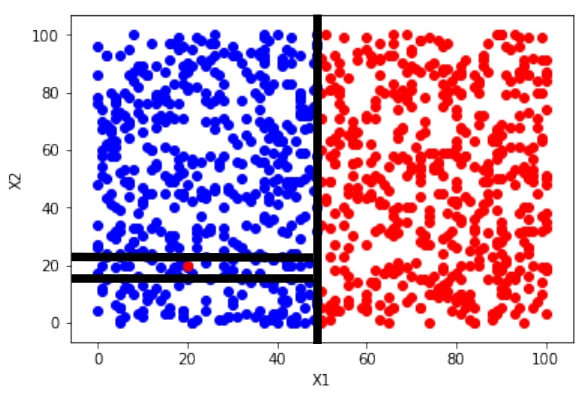
\includegraphics[width=0.6\textwidth]{data_error_cart.jpg}
\caption{Synthetic dataset with CART algorithm splits.}
\label{figure:data_error_cart}
\end{figure}

The tree obtained by applying our algorithm to the dataset of Figigure \ref{figure:data_error_cart} can be seen in Figure \ref{figure:data_error_nes}. The nescience based algorithm does not try to model the error point, since the gain due to an increment in the accuracy does not compensate the surfeit introduced in the model. Recall that the algorithm stops when the total nescience of the tree, based on the measures of miscoding, inaccuracy and surfeit, does not decrease when adding new nodes to the tree. Our algorithm presents a lower sensitivity to the errors found in datasets, at least if the number of errors is small compared with the number of valid points.

\begin{figure}[h]
\centering
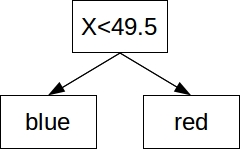
\includegraphics[width=0.4\textwidth]{small_error.jpg}
\caption{Decision tree obtained by the nescience algorithm.}
\label{figure:data_error_nes}
\end{figure}

Our second experiment, again with synthetic dataset, is depicted in Figure \ref{figure:blobs}. There, we create two isotropic Gaussian blobs that partially overlap. We start with a standard deviation of $2.5$ for each cluster, so they are easy to separate, and we increase the standard deviation in increments of $0.01$, until we reach $4.5$, which causes significant overlaps. For each value of the standard deviation, we run the experiment $100$ times and we compute the average accuracy for the two algorithms using different datasets for training (70\% of the data) and testing (30\% of the data). The results of this experiment are shown in Figure \ref{figure:accuracy_blobs}.

\begin{figure}[h]
\centering
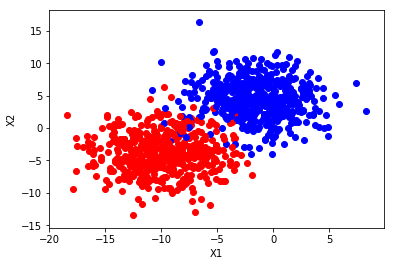
\includegraphics[width=0.6\textwidth]{blobs.png}
\caption{Isotropic Gaussian Blobs.}
\label{figure:blobs}
\end{figure}

As we can see, the performance of both algorithms, in terms of accuracy, is similar. However we should note that the hyperparameter \texttt{minimum\_leaf\_size} of the CART algorithm has been optimized to achieve the best accuracy. For this particular experiment, the best value was achieved with a minimum leaf size of 26 points. By definition, given the fact that CART has one degree of freedom more than the nescicence algorithm, it should produce better accuracy; something that it is not observed (both algorithms have a mean accuracy of $0.87$.

\begin{figure}[h]
\centering
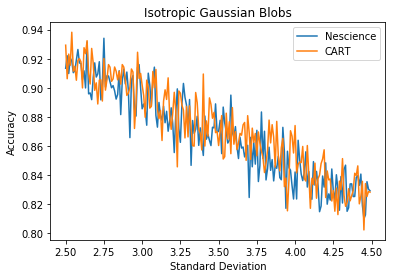
\includegraphics[width=0.6\textwidth]{accuracy_blobs.png}
\caption{Accuracy of Isotropic Gaussian Blobs.}
\label{figure:accuracy_blobs}
\end{figure}

For each iteration of the experiment, we have also computed the average number of nodes, including internal and leaf nodes, required by the models to properly classify the clouds in the dataset. The results of this measurement are show in Figure \ref{figure:length_nodes}. Our algorithm requires an average of $4$ nodes compared to $23$ nodes for the CART algorithm. Moreover, our algorithm is more stable than CART, in the sense that it produces models of similar complexity when it gets similar input datasets (a standard deviation of $0.31$ compared to $3.77$ for CART).

\begin{figure}[h]
\centering
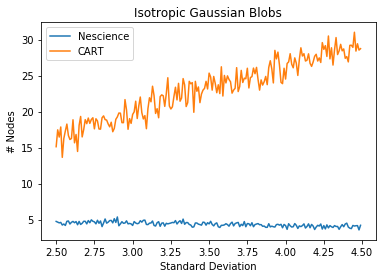
\includegraphics[width=0.6\textwidth]{nodes_blobs.png}
\caption{Number of Nodes.}
\label{figure:length_nodes}
\end{figure}

In Figure \ref{figure:blob_max_depth} we show the maximum depth of the tree, defined as the longest path from the root of the tree to any of its leaves. The maximum depth of the tree is a good measure of the average time it will require for the model to provide a classification. The nescience algorithm has an average depth of $1.6$ nodes, whereas the average depth yielded by the CART algorithm is $4.8$ nodes.

\begin{figure}[h]
\centering
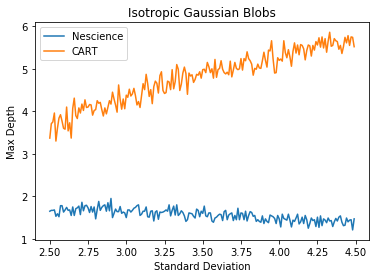
\includegraphics[width=0.6\textwidth]{max_depth.png}
\caption{Maximum depth of the model.}
\label{figure:blob_max_depth}
\end{figure}

The last part of the evaluation consists in comparing the performance of our algorithm and CART with a collection real datasets. More specifically, we have selected $12$ well known datasets from the UCI Machine Learning Repository. The selected datasets are: diagnosis of breast cancer (\texttt{cancer}), optical recognition of handwritten digits (\texttt{digits}), predicting protein localization sites in gram-negative bacteria (\texttt{yeast}), classification of NASA space shuttle data (\texttt{shuttle}), classification of blocks in web pages (\texttt{page}), segmentation of outdoor images (\texttt{image}), predicting the age of abalones from physical measurements (\texttt{abalone}), predicting the quality of red and white variants of Portuguese wine (\texttt{wine}), filter spam emails (\texttt{spam}), wall-following robot navigation (\texttt{wall}), classification of land use based on Landsat satellite images (\texttt{landsat}), and distinguishing signals from background noise in the MAGIC gamma telescope images (\texttt{magic}). For each dataset, we have repeated the experiment 100 times, by randomly selecting the training (70\%) and testing (30\%) subsets at each iteration.

\begin{figure}[h]
\centering
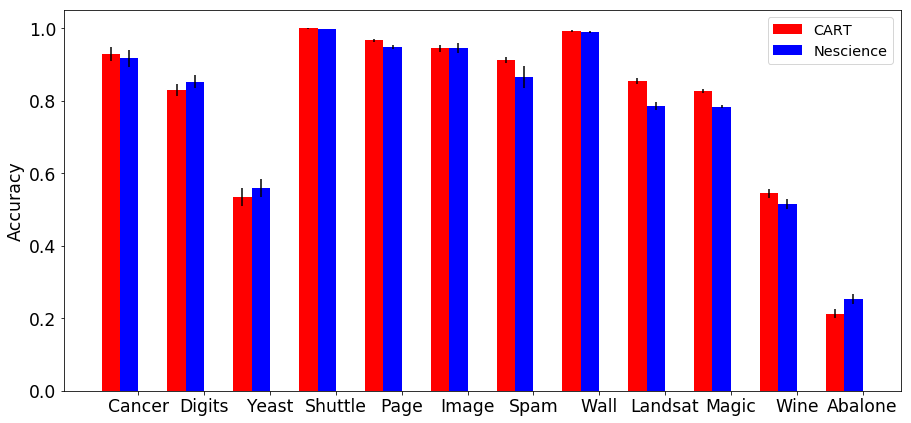
\includegraphics[width=0.6\textwidth]{cart_nescience_accuracy.png}
\caption{Maximum depth of the model.}
\label{figure:cart_nescience_accuracy}
\end{figure}

In Figure \ref{figure:cart_nescience_accuracy} we compare the accuracy of the resulting models obtained by applying the CART algorithm and the nescience algorithm to the above datasets. In $4$ of the $12$ datasets, our algorithm provides better accuracy than CART. In the remaining $8$ cases, the accuracy is, on average, less than $1\%$ smaller.

\begin{figure}[h]
\centering
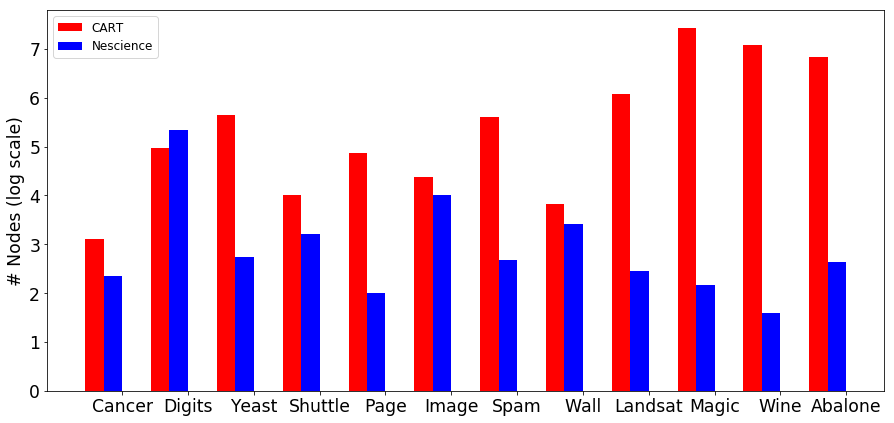
\includegraphics[width=0.6\textwidth]{cart_nescience_nodes.png}
\caption{Maximum depth of the model.}
\label{figure:cart_nescience_nodes}
\end{figure}

In Figure \ref{figure:cart_nescience_nodes} it is shown a comparison of the total number nodes (internal nodes plus leaf nodes) of the resulting models. Only for one of the datasets (\texttt{digits}), our model produces a slightly more complex tree that those generated by CART. In the rest of the cases, the number of nodes in the trees generated by the nescience algorithm have between two and three orders of magnitude fewer nodes (in this figure the $y$ axis is in logarithmic scale).

\begin{figure}[h]
\centering
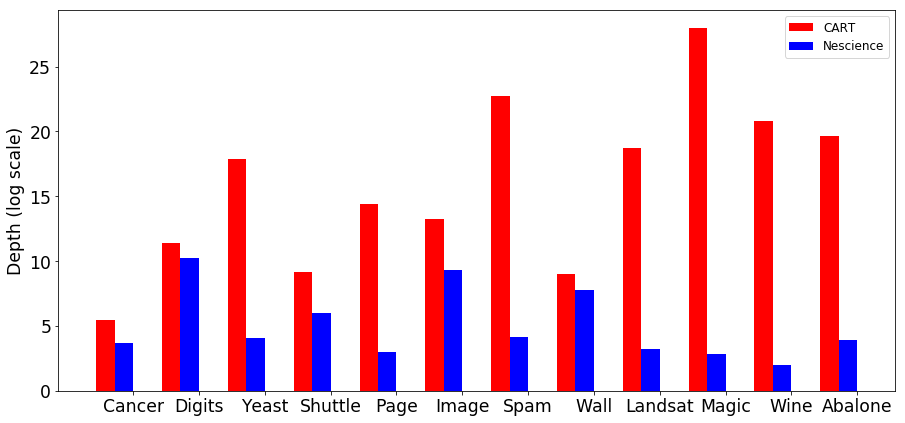
\includegraphics[width=0.6\textwidth]{cart_nescience_depth.png}
\caption{Maximum depth of the model.}
\label{figure:cart_nescience_depth}
\end{figure}

Finally, in Figure \ref{figure:cart_nescience_depth} we provide a comparison of the depth of the tree of the resulting models. Our algorithm always yields a shallower tree than the CART algorithm.

We would like to mention that the nescience algorithm is hihgly robust with respect to the compressor selected or the nescience function implemented. In Table \ref{table:nescience_functions}, we have apply the nescience algorithm to the datasets described above, and evaluate different alternatives for the definition of the nescience function $N (X , M )$: arithmetic mean $(\mu(M , D) + \iota(X , M ) + \sigma(M, D))/3$, geometric mean $(\mu(M , D) + \iota(X , M ) + \sigma(M, D)) 1/3$ , harmonic mean $3 / (\mu(M , D) + \iota(X , M ) + \sigma(M, D)) -1 )$, Euclidean distance $(\mu(M , D) + \iota(X , M ) + \sigma(M, D)) 1/3$, sum $\mu(M , D) + \iota(X , M ) + \sigma(M, D)$, and product $\mu(M , D) + \iota(X , M ) + \sigma(M, D)$. The table shows limited difference between the different functions. 

\begin{table}[h]
\label{table:nescience_functions}
\centering
\begin{tabular}{l l l l l l l l}
\toprule
 & \textbf{Euclid} & \textbf{Arithmetic} & \textbf{Geometric} & \textbf{Product} & \textbf{Addition} & \textbf{Harmonic} \\
\midrule
Accuracy & 0.758 & 0.784 & 0.803 & 0.803 & 0.784 & 0.81 \\
Stdev & 0.051 & 0.041 & 0.033 & 0.033 & 0.041 & 0.038 \\
\bottomrule
\end{tabular}
\caption{Comparison of nescience functions}
\end{table}

Similarly, Table \ref{table:compressor} shows the performance of our algorithm when using the LZMA, zlib, and bz2 compressors. We observe that all of them yield similar performance. The above results suggest that the performance our algorithm is independent of the specific choice made for either implementation aspect.

\begin{table}[h]
\label{table:compressor}
\centering
\begin{tabular}{l l l l}
\toprule
 & \textbf{bz2} & \textbf{lzma} & \textbf{zlib} \\
\midrule
Accuracy & 0.813 & 0.804 & 0.81 \\
Stdev & 0.03 & 0.045 & 0.038 \\
\bottomrule
\end{tabular}
\caption{Comparison of compressors}
\end{table}

We emphasize that the CART algorithm requires to optimize a configuration hyperparameter in order to obtain good results, whereas the algorithm proposed in this book does not require from this optimization.

Shallower trees means faster forecasting times when the models used in production, since the number of \texttt{if-else} conditions to be evaluated is smaller. Moreover, smaller trees makes easier to interpret the results by human analysts. and much shorter training times, something very relevant in case of training ensembles of trees, like random forest or boosted trees (although the use of ensembles of models is highly discouraged by the theory of nescience, given their high surfeit).

%
% Section: Algebraic Model Selection
%

\section{Algebraic Model Selection}

As it was the case for the definition of nescience based on the encyclopedic description of research topics, the nescience of structured datasets can be used to evaluate alternative descriptions of research topics (mathematical models), and to identify how far these descriptions are from an ideal perfect knowledge. This evaluation could be used to identify those topics which require further research. Moreover, the same methodology could be applied to collections of datasets to identify our current knowledge of research areas (collections of topics).

If we combine the concept of nescience of a model, with our concepts of relevance and applicability of research topics, we could apply our methodology for the assisted discovery of interesting questions to collections of datasets; a very useful methodology now that big datasets are becoming widely available.

In order to evaluate the methodology developed, we are going to apply it to a particular research topic: \emph{Multipath Wave Propagation and Fading}. The problem at hand is to understand the effect of a propagation environment on a radio signal, such as the one used by wireless devices. The signals reaching the receiving antenna could follow multiple paths, due to atmospheric reflection and refraction, and reflection from water and objects such as buildings. The effects of these multiple wave paths include constructive and destructive interference (fading), and phase shifting of the original signal, resulting a highly complex received signal (see Figure \ref{fig:Multipath-Signal-Propagation}).

\begin{figure}[h]
\centering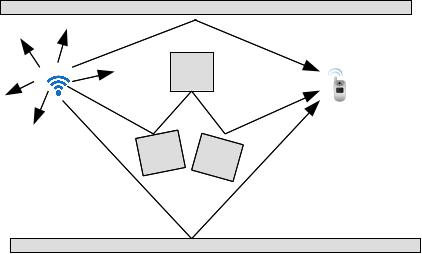
\includegraphics[scale=0.5]{fading}
\caption{\label{fig:Multipath-Signal-Propagation}Multipath Signal Propagation}
\end{figure}

In many circumstances, it is too complicated to describe all reflection, diffraction and scattering processes that determine the different paths the signal will follow. Rather, it is preferable to describe the probability (stochastic model) that the received signal attains a certain value. We are interested in to analyze how well these stochastic models (our current knowledge) are able to describe what happen in reality.

The \emph{Rayleigh fading model} assumes that the magnitude of a signal will vary randomly, or fade, according to a Rayleigh distribution (the radial component of the sum of two uncorrelated Gaussian random variables). The Rayleigh probability density function of the power signal is given by:

\[
P_{\sigma}\left(x\right)=\frac{1}{\sigma}\exp\left[-\frac{x}{\sigma}\right]
\]

where $\sigma$ is the mean of the received signals. Rayleigh fading is viewed as a reasonable model for the effect of heavily built-up urban environments, when there is no dominant propagation along a line of sight between the transmitter and receiver.

The Rice or \emph{Rician distribution} describes the power of the received signal when the target consists in many small scatterers of approximately equal strength, plus one dominant scatterer whose individual received signal equals all that of all the small scatterers combined (there is a dominant line of sight). The probability density function of the power of the received signal is given by:

\[
P(x)=\frac{1}{\bar{\sigma}}\left(1+a^{2}\right)\exp\left[-a^{2}-\frac{x}{\bar{\sigma}}\left(1+a^{2}\right)\right]I_{0}\left[2a\sqrt{\left(1+a^{2}\right)\frac{x}{\bar{\sigma}}}\right]
\]


where $\bar{\sigma}$ is the mean of the received signals, and it is equal to $\bar{\sigma}=\left(1+a^{2}\right)\bar{\sigma}_{R}$, being $a^{2}\bar{\sigma}_{R}$ the power of the dominant scatterer, and $I_{0}$ is the modified zeroth order Bessel function of the first kind.

An experiment (see Figure \ref{fig:Experimental-Set-Up}) was set up to collect a real dataset to analyze. The experiment was run on a $135 m^2$ office full of obstacles (interacting objects). The transmitter was an Odroid C1 Linux computer with a Ralink RT5370 USB Wifi adapter. The receiver was a (fixed in space) Motorla Moto G mobile phone. Data was collected using the Kismet \footnote{https://www.kismetwireless.net/index.shtml} platform (an 802.11 layer2 wireless network detector, sniffer, and intrusion detection system), with some ad hoc, home made, software extensions, mostly for data aggregation. A total of 3,177 samples (power level measured in dBm) were collected during one hour experiment.

\begin{figure}[h]
\centering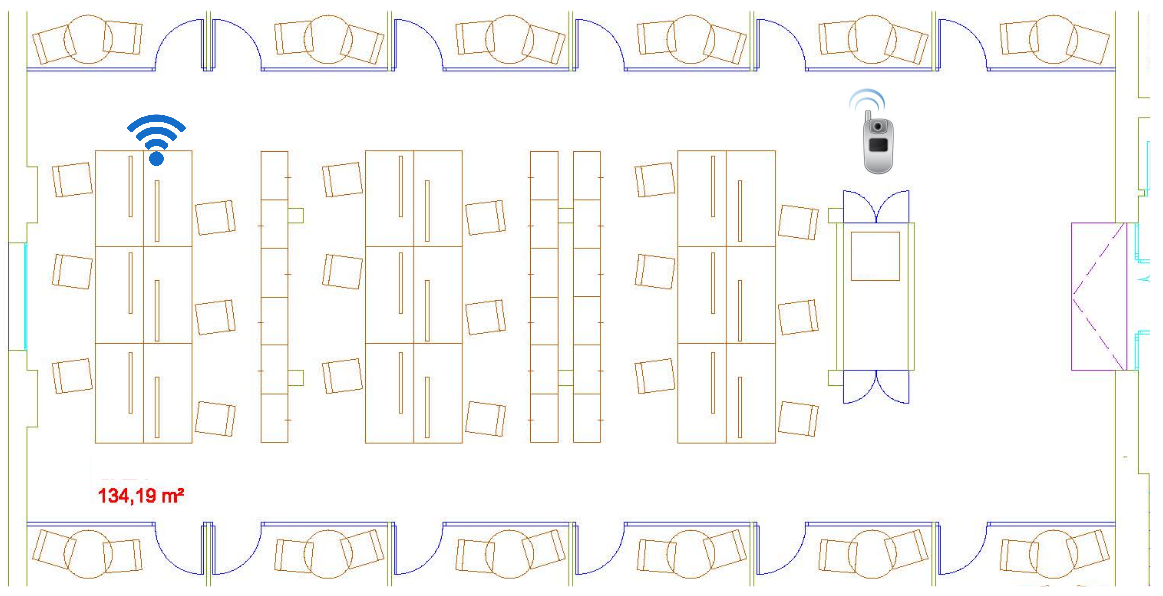
\includegraphics[scale=0.2]{experiment}
\caption{\label{fig:Experimental-Set-Up}Experimental Set Up}
\end{figure}

Next table summarizes the results of applying the three considered models (uniform, Raylegh and Rice) and the optimal encoding using a Huffman code:

\begin{table}[h]
\centering
\begin{tabular}{l l l}
\toprule
\textbf{Model} & \textbf{LDM} & \textbf{Nescience} \\
\midrule
Uniform & 17,351 & 1.30 \\
Rayleigh & 13,229 & 0.75 \\
Rice & 11,118 & 0.47 \\
Huffman & 7,541 & - \\
\bottomrule
\end{tabular}
\caption{Nescience of Models}
\end{table}

The uniform model, that is, assuming zero knowledge about the topic covered by the dataset, has a nescience of 1.30. This value is a kind of upper level for the nescience associated with that particular topic and dataset; any model with a higher nescience should be classified as zero knowledge model. If we introduce the knowledge that in a environment with multiple obstacles the signal propagation can be described as a Gaussian process (Rayleigh distribution), we are able to decrease our nescience to 0.75, that is, there were a 43\% improvement in our understanding of the topic. If we add the knowledge that there is usually a strongly dominant signal seen at the receiver caused by a line of sight between the antenna and the mobile phone (Rician distribution), the nescience decreases to 0.47, and so, we have achieved an additional 23\% gain in our understanding. Given that numbers we can conclude that the Rayleigh model increases our knowledge with respect to the uniform model, and that the Rice model does so with respect to Rayleigh. However, the nescience of this last model is 0.47. That means that there still patterns in the dataset that are not explained by the Rice model, or what it is equivalent according to our methodology, there is still some knowledge to discover and learn.

The methodology has been applied to a dataset gathered in a single experiment under a controlled environment, since the goal of this Chapter was to provide a methodology to quantify the nescience of structured datasets, not to evaluate models for signal propagation and fading. In order to to conclude that, in general, the Rice model is an improvement over Rayleigh, a more realistic experiment is required, with multiple datasets gathered in real environments.

%
% Section: The Analysis of the Incompressible
%

\section{The Analysis of the Incompressible}

As we have said in Chapter {chap:Introduction}, one of the reasons to understand how things work is to understand the cause-effect relation in systems. We are interested in this cause/effect relation in two ways. That is, if we want to see an effect in a system, we want to understand wich causes trigger that effect. Also, and perhaps more interesting, if we have observed an (probably undesired effect) in a system we would like to discover what has caused that effect, so we can fix it, and revert the normal situation.

We could use the theory of nescience to model, and modify, those uncommon effect, by means of training a model and looking at the incompressible part of the data.


A model $\mathcal{M}$ for a dataset $\mathcal{D} = (X, y)$ is a compressed version of that dataset, since the length of the dataset given the model $l(\mathcal{D} \mid \mathcal{M})$ is smaller that then length of the original dataset $l(\mathcal{D})$. The model $\mathcal{M}$ is composed by the regularities found in the dataset (subject to the algorithm used and the families of models considered). What it is left, $\mathcal{D} \mid \mathcal{M}$ is the incompressible part of the dataset, that is, those samples that have no regularity at all, or present a regularity that requires a description longer than the length of the raw data.

In this section we are going to show the practical applications of analyzing what it is left, that is, the incrompressible samples of a dataset. An element that is incompressible represents a very unlikely, or uncommon, situation of the entity being studied. A incompressible element does not necessarily means a problem, since if a problem is sufficiently common, it can be compressed. An incompressible element is something than cannot be explained given the normal behaviour of the system. Of course, all of this is assuming that our dataset has no errors.

Once we have found a model that has the lowest possible nescience for a dataset, we could separate those elements that have not been compresed, denoted by XX, and fit a second model. We could argue that it does not make any sense to model the incompressible part, since, it is incompressible. However, the incompressible part is incompressible with respect to the original entity under study, that is, the global systen. And in this new case, we are studying a different entity, namely, the uncommon parts of an entity. It might happen that we can find regularities in this new entity.



%
% Section: References
%

\section*{References}
\label{sec:ML_references}

A insightful description of the differences between explanation models and predictive models, how these models are used in different scientific disciplines, and what are the implications for the process of statistical modeling can be found in \cite{shmueli2010explain}.

The application of the minimum description length principle to the identification of optimal decision trees have been proposed in \cite{quinlan1989inferring}, further refined and clarified in \cite{wallace1993coding}; however the coding method proposed by those authors is different from the one used in this book.

In our web page can be found an implementation of the decision tree following the guidelines defined in []. 


The Minimum Description Length \cite{grunwald2007minimum} and the Minimum Message Length \cite{wallace2005statistical} techniques have been applied to the problem of inferring decision trees in \cite{quinlan1989inferring}, later on clarified and extended in~\cite{wallace1993coding}, in \cite{mehta1995mdl} as a technique for pruning, and in \cite{rastogi1998public}, among others. Although the underlining concepts behind the cost function proposed in this chapter are the same (namely, that learning is equivalent to the capability to compress), our approach is very different from the ones described in these works.

An excellent survey of the available discretization methods can be found in~\cite{garcia2013survey}; in the paper the authors also propose a taxonomy to classify existing methods based in their properties and they conduct an extensive comparative experimental study. The proportional discretization method used to compute miscoding is introduced in~\cite{yang2009discretization}, where there is also a theoretical justification of why this method reduces the bias and the variance of the discretized variable.

{\color{red} TODO: Find the original reference of the AirPassengers dataset.}

{\color{red} TODO: Find the original reference of the Appliance energy consumption dataset. https://archive.ics.uci.edu/ml/datasets/Appliances+energy+prediction}



